\documentclass[12pt]{My_preprint}
\title{
    %First moment of hydrodynamic forces on a translating spherical droplet immersed in a uniform flow at low but finite inertia effects.
    Rheology of a suspension made of non-buoyant spherical droplets
    }

\author[1,2]{Nicolas Fintzi and  Jean-Lou Pierson}

\normalmarginpar


\begin{document}

\maketitle

\begin{abstract}
    In this note, we use the reciprocal theorem to compute the first moment of hydrodynamic forces applied on a translating spherical droplet immersed in a uniform flow. 
    According to Hadamard-Rybczynski solution \citep{kim2013microhydrodynamics}, the first moment generated by the flow field surrounding a translating spherical droplet in a uniform flow, in the Stokes regime, is identically null. 
    In this study we consider finite but low droplet Reynolds number, $Re$, and compute the first order correction in $Re$ of the first moment of hydrodynamic forces. 
    It is shown that, in dimensionless form, the first moment is proportional to the square of the relative velocity times the Reynolds number.  
    The main consequence of that finding is that in a dilute emulsion of buoyant droplets, the effective stress is also proportional to the relative motion between phases and the Reynolds number. 
    % Particularly, we show that this stress have the form $\sim Re\phi [C_1\textbf{UU}+C_2\textbf{U}\cdot\textbf{U}]$ where $C_1$ and $C_2$ are constant of order one, and $\phi$ is the volume fraction. 
\end{abstract}


\section{Introduction}

To better illustrate the role of various forces and stresses in a multiphase flow model, we begin by presenting the averaged momentum equations for the dispersed and continuous phases, derived through an ensemble averaging procedure.
For mono-disperse emulsions, the mass and momentum equations of the continuous phase and dispersed phase can be written as \citep{fintzi2024averaged},
\begin{align}
    % \phi_f + \phi &= 1\\
    (\pddt + \textbf{u}_f  \cdot \grad) \phi_f
    &= - \phi_f \div \textbf{u}_f\\
    (\pddt + \textbf{u}_p \cdot \grad)n_p
    &=
    - n_p \div \textbf{u}_p\\
    m_pn_p (\pddt + \textbf{u}_p \cdot \grad)\textbf{u}_p
    % + \div \pavg{m_p \textbf{u}_\alpha'\textbf{u}_\alpha'}
    &=
    n_pm_p(\div \bm\Sigma
    + \rho_d  \textbf{g})
    + \div \bm\sigma_p^\text{eff}
    + n_p\textbf{f}_p
    \\
    \phi_f \rho_f(\pddt + \textbf{u}_f  \cdot \grad) \textbf{u}_f
    &= \phi_f 
    \left(\div \bm{\Sigma}
    + \rho_f \textbf{g}\right)
    + \div \bm\sigma_f^{\text{eff}}
    - n_p\textbf{f}_p
    \label{eq:dt_uf2}
\end{align}
respectively. 
The subscript $f$ and $p$ refer to continuous phase and droplets phase averaged quantities, respectively.
The vector $\textbf{g}$ is the acceleration of gravity and $\rho_k$ is the density of the phase $k$. 
$\phi_f$ is the volume fraction of the continuous phase, $n_p$ the particle number density.
In the following we use the notation $\phi \to n_p v_p$, with $v_p$ the mean volume of droplet.
$\textbf{u}_f$ (resp. $\textbf{u}_p$) is the averaged velocity of the fluid (resp. dispersed) phase, $\bm\Sigma = - p_f \bm\delta + \mu_f [\grad \textbf{u} +  (\grad \textbf{u})^\dagger ]$ the \textit{mean Newtonian stress} of the mixture, with $p_f$ being the mean hydrodynamic pressure and $\textbf{u}=\phi_f \textbf{u}_f + \phi \textbf{u}_p$ the volume averaged velocity of the mixture.
$\bm{\sigma}^{\text{eff}}_p$ and $\bm{\sigma}^{\text{eff}}_f$ are the effective stresses of the dispersed and continuous phase, respectively.  
Finally, $\textbf{f}_p$ represents the interphase momentum exchange, or drag force density term. 

The number density, continuous phase volume fraction, drag force density, and effective stresses of the dispersed and continuous phase, can be expressed formally as,
\begin{align}
    n_p &= \pavg{}
    \label{eq:n_p}\\
    \phi_f &= \avg{\chi_f}
    \label{eq:chi_f}\\
    n_p \textbf{f}_p  &= \pSavg{\bm\sigma^*_f\cdot \textbf{n}}
    \label{eq:f_alpha}
    \\
    \bm{\sigma}_p^{\text{eff}} &= \pavg{\textbf{u}_\alpha'\textbf{u}_\alpha'}
    \label{eq:def_uup}
    \\
    \bm{\sigma}^{\text{eff}}_f 
    &= 
    - \avg{\chi_f\rho_f \textbf{u}_f'\textbf{u}_f'} 
    + \pavg{\intS{\textbf{r}\bm\sigma^{*}_f\cdot \textbf{n}} - \delta_p\intO{2\mu_f\textbf{e}_d^*}}\nonumber\\
    &- \div
        \pavg{ \frac{1}{2}\intS{\textbf{rr}\bm\sigma^{*}_f\cdot \textbf{n}}
        - \delta_p\intO{2\mu_f \textbf{r} \textbf{e}_d^*}}
        + \grad\grad (\ldots). 
    \label{eq:def_sigma_eff_f}
\end{align}
respectively. 
Where the operator $\avg{\ldots}$ corresponds to an ensemble average procedure, 
$\textbf{u}_\alpha$ is the center of mass velocity of a particle labeled $\alpha$, $\chi_f$ is the phase indicator function of the continuous phase, and $\delta_p$ the Dirac delta function pointing on the particle center of mass, $\delta_\Gamma$ the interfaces' indicator function, and \textbf{n} the normal of the surface pointing outward the droplets. 
The superscript $'$ indicates the relative values of a quantity with respect to its phase-averaged value. 
Specifically $p_f' = p_f^0 - p_f$, $\textbf{u}_\alpha' = \textbf{u}_\alpha - \textbf{u}_p$ and $\textbf{u}_f' = \textbf{u}_f^0  -\textbf{u}_f$, with $\textbf{u}_f^0$,  the local velocity of the continuous phase, respectively. 
The superscript $^*$ represents the relative values of a quantity with respect to the mixture volume averaged value, such that $\bm{\sigma}_f^* = \bm{\sigma}_f^0  - \bm{\Sigma}$ and $\textbf{e}_d^* = \textbf{e}_d^0 - \textbf{E}$ with $\bm{\sigma}_f^0 = -p_f^0 + \mu_f [\grad \textbf{u}_f^0 + (\grad \textbf{u}_f^0)^\dagger]$ the local stress of the continuous phase. 




In the present situation the ``closure problem'' consists in finding explicit expressions for the terms of the form $\avg{\ldots}$, in \ref{eq:f_alpha}, \ref{eq:def_uup} and \ref{{eq:def_sigma_eff_f}}, in terms of the unknown of the problem, i.e. $n_p$, $\phi_f$, $p_f$, $\textbf{u}_p$ and $\textbf{u}_f$. 
In this work we focus on the last two terms of $\bm\sigma^\text{eff}_f$, i.e. the first and second moment of hydrodynamic forces acted upon spherical droplets.
Hence, one must find an expression for the disturbance fields $\bm\sigma_f^*$ evaluated at the surface of a test droplet and of the field $\textbf{e}_d^*$ inside the test droplet. 
Because they are evaluated at the surface and in the interior of the test droplets, these terms may be written as, 
\begin{align}
    \bm\sigma_f^* =p_f' \bm\delta 
    + \mu_f [\grad \textbf{u}^* + (\grad \textbf{u}^*)^\dagger]
    && 
    \textbf{e}_d^* = [\grad \textbf{u}^* + (\grad \textbf{u}^*)^\dagger] /2
\end{align}
with $\textbf{u}^* = \textbf{u}^0 - \textbf{u}$ and $\textbf{u}^0$ the local velocity of the mixture, which becomes $\textbf{u}_d^0$ inside the test droplet and $\textbf{u}_f^0$ at the surface of the fluid droplet. 

We limit this theoretical investigation to dilute suspension. 
Likewise, we consider only vanishingly small, but non-zero, values of the droplet Reynolds number, defined as,
\begin{equation}
    Re  = \frac{|\textbf{u} - \textbf{u}_p|\rho_f a}{\mu_f}, 
\end{equation}
where $a$ is the radius of the droplets. 
Consequently, the values of $\bm\sigma_f^*$ and $\textbf{e}_d^*$ will only be accurate at order $O(1)$ in the volume fraction (neglecting the droplets interactions) and $O(Re)$ in the Reynolds number. 
Hence, after integration over the surface of the droplet and ensemble averaging these terms will bring a contribution of $O(Re \phi)$ in the averaged momentum equation. 
Note that in the following we consider arbitrary density and viscosity ratio,
\begin{align}
    \lambda = \mu_d/\mu_f,  && \zeta =\rho_d /\rho_f,
\end{align}
where $\mu_d$ and $\rho_d$ are the viscosity and density of the droplets.

In the following we revisit the methodology of \citet{stone2001inertial,raja2010inertial,dabade2015}  to compute the first moment of force on a spherical droplet embedded in a uniform flow at low but finite inertia effects. 
In opposition to \citet{stone2001inertial} and \citet{raja2010inertial} who considered neutrally-buoyant sherical inclusion embedded in a shear flow, we focus on the relative motions of droplets with the continuous phase. 
\citet{dabade2015} computed the torque (skew-symmetric part of the first moment) on a spheroidal particle embedded in a uniform flow. 
Our study is similar to the work of \citet{dabade2015}, however we aim to compute the whole first moment tensor (not only the torque), and we consider droplets (instead of solid spheroidal particles). 
Therefore, we propose an original method, mainly inspired from \citet{stone2001inertial}, to compute the first moment of force on droplets at first order $Re$.  

\tb{The second objectif of this study is to propose a general formula of the reciprocal theorem to allows extension of these results in future study}
% \section{The reciprocal theorem and equaitons for a droplet force and Stresslet}
% \label{ap:reciprocal}




\section{Governing equations and fundamentals solutions}
\label{sec:governing_equation}

At the leading order in droplet volume fraction, the governing equations for $\textbf{u}^*$ and $p_f'$ are equivalent to that of an isolated droplet immersed in an infinite medium \citep{hinch1977averaged}. 
Hence, we consider the problem of an isolated test droplet immersed in an arbitrary flow where only the uniform relative motions induce inertia. 
The disturbances pressure and velocity fields ($\textbf{u}^*$ and $p_f'$), relative to the position of a test droplet are noted $\textbf{u}_{o}$, $\textbf{u}_{i}$, $p_{o}$ and $p_{i}$, for the velocity outside, and inside, the pressure outside and inside the volume of the test droplet, respectively. 
Recall that the center of mass velocity of the droplet is noted $\textbf{w}$. 
On~\ref{fig:disturbance} we display a schematic representation of the problem. 
\begin{figure}[h!]
    \centering
    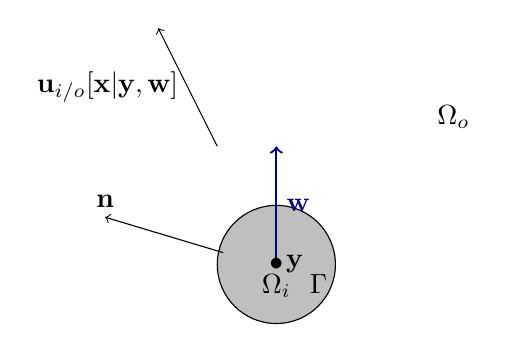
\begin{tikzpicture}[scale= 1.5]
        \filldraw[ gray!50!white](0,0)circle (0.5);
        \draw(0,0)circle (0.5)node[right,below]{   $\;\;\;\;\;\;\;\;\;\;\;\Gamma$};
        \draw[->,blue!50!black,thick](0,0)--++(0,1)node[midway,right]{$\textbf{w}$};
        \draw (0,0)node{$\bullet$}node[right]{$\textbf{y}$};
        \draw[->] (-0.45,0.1)--++(-1,0.3)node[above]{$\textbf{n}$};
        \draw[->](-0.5,1)--++(-0.5,1)node[midway,left]{$\textbf{u}_{i/o}[\textbf{x}|\textbf{y},\textbf{w}]$};
        % \draw[->] (3,1)node{$\bullet$}--++(0,1.5)node[right,midway]{$\textbf{u}_f[\textbf{x}]$};
        \draw (0,0)node[below]{$\Omega_i$};
        \draw (1.5,1.25)node{$\Omega_o$};
    \end{tikzpicture} 
    \caption{Representation of the problem parameters. $\textbf{u}_{o/i}[\textbf{x}|\textbf{y},\textbf{w}]$ is the disturbance velocity field evaluated at \textbf{x}, generated by a test droplet positioned at \textbf{y} with center of mass velocity \textbf{w}. \textbf{n} is the unit normal  pointing outward the droplet. 
    The domain of the exterior of the droplet is noted $\Omega_o$ and the one the interior $\Omega_i$.}
    \label{fig:disturbance}
\end{figure}

\subsection{Maxey, Riley \& Gatignol's equations}

Outside and inside the volume of the test droplet we can write the mass and momentum equations for the disturbances fields, that we noted $p_{o/i}$ and $\textbf{u}_{o/i}$, by conditionally averaging the Navier stokes equations \citep{koch1993hydrodynamic,fintzi2025}, or simply by considering the equations derived by~\cite{maxey1983equation} \& \citet{gatignol1983faxen}, both approach are equivalent\footnote{
    It must be noted that even in dilute systems, conditional averaging induces an additional stress in~\ref{eq:momentum_out} (see~\cite[Eq. (9)]{koch1993hydrodynamic}), which is not present in~\cite{maxey1983equation} \& \citet{gatignol1983faxen}'s equations. 
    This term corresponds to the velocity variance of the conditionally averaged velocity field (see \citet{koch1993hydrodynamic} or \citet[Chapter 4]{fintzi2025}), it is similar to the Reynolds Stress. 
    However, in this work, the turbulence considered is only the ``pseudo-turbulence'', hence it is $\propto \phi$ to some power. 
    Hence, in the conditionally averaged equations, this term turns out to be negligible \citep[Appendix A]{koch1993hydrodynamic}.
    In this context, conditionally averaged equations are equivalent to the equations for an isolated droplet. 
    The only difference is that conditionally averaged equations are explicitly related to ensemble averaged fields through their boundary conditions \citep{fintzi2025}. 
}. 
In dimensionless form they read, 
\begin{align}
    \div \textbf{u}_{o} &= 0
    \\
    \div\bm\sigma_{o}
    &= 
    Re [
    \pddt \textbf{u}_{o}
    + \textbf{u}_{o}\cdot \grad \textbf{u}_{o}
    + \textbf{u}_{o}\cdot \grad \textbf{w}_r
    + \textbf{w}_r \cdot \grad \textbf{u}_{o}]
    = Re \textbf{f}_{o},
    \label{eq:momentum_out}
\end{align}
for all $|\textbf{x}- \textbf{y}| = |\textbf{r}| = r > 1$, and, 
\begin{align}
    \div \textbf{u}_{i} &= 0,
    \\
    \div\bm\sigma_{i}
    &= 
    \frac{\zeta}{\lambda}Re [
    \pddt \textbf{u}_{i}
    + \textbf{u}_{i}\cdot \grad \textbf{u}_{i}
    + \textbf{u}_{i}\cdot \grad \textbf{w}_r 
    + \textbf{w}_r \cdot \grad \textbf{u}_{i}]
    = \frac{\zeta}{\lambda}Re \textbf{f}_{i},
    \label{eq:momentum_in}
\end{align}
for $r<1$. 
Here we introduced the notation $\textbf{w}_r = \textbf{u} - \textbf{w}$.  
We recall here that \textbf{u} is the undisturbed, or ensemble averaged velocity, governed by the ensemble averaged equations (from~\ref{eq:dt_phif} to~\eqref{eq:dt_uf2}).
Additionally, $\bm\sigma_{i/o} = -p_{i/o}\bm\delta + 2\textbf{e}_{i/o}$ with $\textbf{e}_{i/o} = \frac{1}{2}[\grad \textbf{u}_{i/o} + ^{\dagger}\grad \textbf{u}_{i/o}]$ is the dimensionless newtonian stresses in the interior and exterior of the test droplet. 
% We introduce the Reynolds number $Re = \frac{\rho_f a |\textbf{w}_r|}{\mu_f}$ based on the droplet radius $a$, the density ratio $\zeta = \rho_d / \rho_f$ and the viscosity ratio $\lambda = \mu_d / \mu_f$. 
Note that the distances have been made dimensionless using the radius $a$, and the velocities using the scale $U = |\textbf{w}_r|$, and the stresses using the scale $U\mu_f /a$. 
Because we neglected inertial effects generated due to linear and quadratic flows, as well as unsteady behaviors, the first and third term on the right-hand side of~\ref{eq:momentum_in,eq:momentum_out} will cancel in the calculation performed in~\ref{sec:compute_moments}. 


At the surface of the droplet ($r = 1$) the continuity of velocity and the non-deformability of the test droplet imposes, 
\begin{align}
    \textbf{u}_{i} - \textbf{u}_{o}= 0,
    && 
    (\textbf{u}_{i}+\textbf{w}_r) \cdot \textbf{n}
    =
    0.
    \label{eq:normal_vel}
\end{align} 
At the interface of the test droplet the absolutes tangential shear rates ($\textbf{e}_{i/o}+\textbf{E}$) are assumed continuous, however the disturbance shear rate $\textbf{e}_{i/o}$ is not. 
Recall that $\textbf{E} =\frac{1}{2} [\grad \textbf{u} + ^\dagger \grad \textbf{u}]$ is the ensemble averaged shear rate of the continuous phase.
Hence, the correct boundary condition for the disturbance shear rate is (at $r=1$),
\begin{equation}
    \mathbf{n}\cdot 2 [\textbf{e}_{o} - \lambda \textbf{e}_{i} + (1-\lambda)\textbf{E}
    % - \textbf{b}
    ]\cdot (\bm\delta - \textbf{nn})
    =
    \textbf{b}\cdot (\bm\delta - \textbf{nn}),
    % 0
    \label{eq:boundary_cdt_stress}
\end{equation}
with, 
\begin{equation}
    \textbf{b}
    =
    \frac{a \grad \gamma}{\mu_f |\textbf{w}_r|}. 
    % = Ma \grad\gamma /|\grad \gamma|. 
\end{equation}

Here we have considered Marangoni stresses in order to keep general when deriving the reciprocal relation (see~\ref{sec:reciprocal}), nevertheless $\textbf{b}$ will be taken to be zero in the final calculation of the moments \eqref{sec:compute_moments}. 
Note that for instance the ensemble averaged quantities $\textbf{u}$ and $\textbf{E}$ are kept general, hence their values depends on the position along the surface of the test droplet, thus $\textbf{w}_r[\textbf{r}]$ isn't a constant of space. 



Far from the test droplet it is assumed that the disturbance fields are statistically independent form the presence of the droplet, hence we have the following boundary condition far form the test drop,  
\begin{align}
    \lim_{r \to\infty }\textbf{u}_{o}[\textbf{r}|\textbf{y},\textbf{w}] = 0,
    && \lim_{r \to\infty }p_{o}[\textbf{r}|\textbf{y},\textbf{w}]= 0. 
    \label{eq:BC_r_infty_1}
\end{align}





\subsection{Stokes flow solution for a droplet embedded in a quadratic flow}
The Reciprocal theorem requires the use of a known solution.
We call that solution the \textit{test} solution, since its only purpose is to compute the \textit{real} solution of the equations introduced above. 
We note the \textit{test} velocity and stress fields $\hat{\textbf{u}}_{i/o}$ and $\hat{\bm\sigma}_{i/o} = - \hat{p}_{i/o}\bm\delta + \grad \hat{\textbf{u}}_{i/o} + ^\dagger\grad \hat{\textbf{u}}_{i/o}$, respectively. 
In general all the \textit{test} quantities are written with a hat. 

In this problem we neglect all inertial effects and consider an arbitrary quadratic flow. 
In this situation $\hat{p}_{o/i}$ and $\hat{\textbf{u}}_{o/i}$ satisfy,
\begin{align}
    \div \hat{\textbf{u}}_{o} = 0 
    &&\div\hat{\bm\sigma}_{o}  = 0 
    \label{eq:momentum_out_s}\\
    \div \hat{\textbf{u}}_{i} = 0 
    && \div\hat{\bm\sigma}_{i}  = 0 
    \label{eq:momentum_in_s}
\end{align}
with the boundary conditions, 
\begin{align}
    \lim_{r \to\infty }\hat{\textbf{u}}_{o}[\textbf{r}|\textbf{y},\textbf{w}] = 0,
    && \lim_{r \to\infty }\hat{p}_{o}[\textbf{r}|\textbf{y},\textbf{w}]= 0. 
    \label{eq:BC_r_infty_2}
\end{align}
and (at $r=1$),
\begin{align}
    \label{eq:normal_vel2_s}
    \hat{\textbf{u}}_{i} &= \hat{\textbf{u}}_{o}\\
    \hat{\textbf{u}}_{i} \cdot \textbf{n} &= - \hat{\textbf{w}}_r \cdot \textbf{n}
    \label{eq:normal_vel_s}
    \\
    \label{eq:normal_stres_s}
    \mathbf{n}\cdot 2[\hat{\textbf{e}}_{o} - \lambda \hat{\textbf{e}}_{i} + (1-\lambda) \hat{\textbf{E}}
    % - \hat{\textbf{b}}
    ]\cdot (\bm\delta - \textbf{nn})
    &=
    \hat{\textbf{b}}\cdot (\bm\delta - \textbf{nn})
    % 0
\end{align}
where we introduced $\hat{\textbf{w}}_r = \hat{\textbf{u}} - \textbf{w}$ as the undisturbed relative velocity field of the test problem, similarly $\hat{\textbf{E}}$ is the undisturbed stress of the test problem. 
Note that for the test problem it is important that $\hat{\textbf{b}}\neq 0$, this will be useful to write the reciprocal relation in~\ref{sec:reciprocal}.


For our purposes we only need $\hat{\textbf{b}}$ and $\hat{\textbf{u}}$ to be quadratic fields.
Hence, we consider the relations, 
\begin{align}
    \hat{\textbf{w}}_r(\textbf{y} + \textbf{r}) 
    &=  \hat{\textbf{w}}_r|_{\textbf{r}=0}
    +  \textbf{r} \cdot  \grad\hat{\textbf{u}}|_{\textbf{r}=0}
    +  \frac{1}{2}\textbf{rr} :  \grad\grad\hat{\textbf{u}}|_{\textbf{r}=0}
    \label{eq:w_r_expand}\\
     \hat{\textbf{E}}(\textbf{y} + \textbf{r}) 
    &=   \hat{\textbf{E}}|_{\textbf{r}=0}
    + \textbf{r} \cdot  \grad \hat{\textbf{E}}|_{\textbf{r}=0}
    %+ \frac{1}{2}\textbf{rr} :  \grad\grad \hat{\textbf{E}}|_{\textbf{r}=0}
    \\
     \hat{\textbf{b}}(\textbf{y} + \textbf{r}) 
    &=   \hat{\textbf{b}}|_{\textbf{r}=0}
    + \textbf{r} \cdot  \grad \hat{\textbf{b}}|_{\textbf{r}=0}
    + \frac{1}{2}\textbf{rr} :  \grad\grad \hat{\textbf{b}}|_{\textbf{r}=0}
\end{align}
% \tb{note that we don't consider the symmetry between gradient hence $\grad\grad\hat{\textbf{u}}\approx $ arbitrary tensor; this is already what is considered }

According to the linearity of the Stokes equations~\ref{eq:momentum_out_s,eq:momentum_in_s}, and of the boundary conditions~\ref{eq:normal_vel2_s,eq:normal_vel_s,eq:normal_stres_s} we deduce that $\hat{\textbf{u}}_{i/o}$ and $\hat{p}_{i/o}$  must be linear combination of spherical harmonics proportional to $\hat{\textbf{w}}_r|_{\textbf{r}=0}$, $\hat{\textbf{b}}|_{\textbf{r}=0}$, and their derivatives \citep{brenner1963resistance}.
Hence, we can write the general solution of $\textbf{u}_{i/o}$ and $p_{i/o}$ as,
\begin{align}
    \begin{pmatrix}
        \hat{\textbf{u}}_{o}\\
        \hat{p}_{o}\\
        \hat{\textbf{u}}_{i}\\
        \hat{p}_{i}
    \end{pmatrix}
    =
    \begin{pmatrix}
        \textbf{U}_{o}^{(1)} + \textbf{U}_{o}^{(2)}\cdot \grad + \textbf{U}_{o}^{(3)} :\grad\grad &
        \textbf{U}_{o}^\text{(1-b)} + \textbf{U}_{o}^\text{(2-b)}\cdot \grad + \textbf{U}_{o}^\text{(3-b)} :\grad\grad \\
        \textbf{P}_{o}^{(1)} + \textbf{P}_{o}^{(2)}\cdot \grad + \textbf{P}_{o}^{(3)} :\grad\grad &
        \textbf{P}_{o}^\text{(1-b)} + \textbf{P}_{o}^\text{(2-b)}\cdot \grad + \textbf{P}_{o}^\text{(3-b)} :\grad\grad \\
        \textbf{U}_{i}^{(1)} + \textbf{U}_{i}^{(2)}\cdot \grad + \textbf{U}_{i}^{(3)} :\grad\grad &
        \textbf{U}_{i}^\text{(1-b)} + \textbf{U}_{i}^\text{(2-b)}\cdot \grad + \textbf{U}_{i}^\text{(3-b)} :\grad\grad \\
        \textbf{P}_{i}^{(1)} + \textbf{P}_{i}^{(2)}\cdot \grad + \textbf{P}_{i}^{(3)} :\grad\grad &
        \textbf{P}_{i}^\text{(1-b)} + \textbf{P}_{i}^\text{(2-b)}\cdot \grad + \textbf{P}_{i}^\text{(3-b)} :\grad\grad \\
    \end{pmatrix}
    \cdot 
    \begin{pmatrix}
        \hat{\textbf{w}}_r\\
        \hat{\textbf{b}}
    \end{pmatrix}
    \label{eq:big_solution}
\end{align}
The tensor $\textbf{U}_{i/o}^{(n)}$ and $\textbf{P}_{i/o}^{(n)}$ are $n+1$ and $n$ order tensors given in \citet[Appendix F]{fintzi2025averaged}, that depend only on the relative coordinate $\textbf{r} = \textbf{x}-\textbf{y}$ and the viscosity ratio $\lambda$.
We also define the $n+2$ order tensors, 
\begin{equation}
    \textbf{S}_{i/o}^{(n)} = 
    - \bm\delta\textbf{P}_{i/o}^{(n)}
    + \grad \textbf{U}_{i/o}^{(n)}
    + ^\dagger\grad \textbf{U}_{i/o}^{(n)},
    \label{eq:big_S}
\end{equation}\footnote{The $^\dagger$ used in~\ref{eq:big_S} represents the transpose operator which acts on the two closet index.
For example, the transpose of the triadic $\textbf{abc}$, may be written:  $^\dagger\textbf{abc} = \textbf{bac}$ or $\textbf{abc}^\dagger = \textbf{acb}$. }
where $n =1,2,3$ or $1\text{-}b,2\text{-}b,3\text{-}b$. 
\ref{eq:big_S} provides the stresses fields of the test problem upon contraction with $\hat{\textbf{w}}_r$, and $\hat{\textbf{b}}$, and the higher derivatives. 

\subsection{Singularity solutions}

Following \citet{stone2001inertial} we also consider the test problem of a point source located at the origin.
The reason why this solution is necessary is because, in the previous test problem $\div \hat{\textbf{u}}= 0$, hence the previous solution was unable to provide a formula for the trace of the first moment using the reciprocal theorem.
Because we also aim to compute the traces of the second moment of force one also need solution of point forces and potential dipole.  
These two classes of solutions, i.e., point force and point source, obey   the non-homogeneous Stokes equations, 
\begin{align}
    \grad^2 \hat{\textbf{u}}_o = \grad \hat{p}_o + (\textbf{Q}^{(n)}\otimes \grad^{(n)})\grad \delta(\textbf{r}),
    &&
    \grad^2 \hat{\textbf{u}}_o = \grad \hat{p}_o + (\textbf{B}^{(n+1)}\otimes \grad^{(n)}) \delta(\textbf{r}),
\end{align}
respectively. 
Where $\textbf{Q}^{(n)}$ and $\textbf{B}^{(n+1)}$ are two arbitrary $n^{th}$ and $(n+1)^{th}$ order tensors, respectively. 
Similarly the $\grad^{(n)}$ denote $n^{th}$ order outter product of gradients vectors.
The operator $\otimes$ represents the contraction product on the $n^{th}$ common indices. 
Both equations are completed by the continuity equation $\div \textbf{u}_{o}$. 
The solution of the point source, and point forces equations read, 
\begin{align}
    \hat{\textbf{u}}_o = -\frac{1}{4\pi}\grad^{(n+1)}(1/r)\otimes \textbf{Q}^{(n)}
    \label{eq:pts_source_n}
    &&
    \hat{\textbf{u}}_o = \frac{1}{8\pi}\grad^{(n)}[\grad^{(2)} - \bm\delta \grad^2]r
    \otimes \textbf{B}^{(n+1)}
\end{align}
The Stresses tensors read, 
\begin{align}
    \hat{\bm\sigma}_o = -\frac{1}{2\pi}\grad^{(n+2)}(1/r)\otimes \textbf{Q}^{(n)}, 
    &&
    \hat{\bm\sigma}_o = \frac{1}{8\pi}\grad^{(n)}[
        2\grad^{(3)}
        -(\grad \bm\delta + ^\dagger\grad\bm\delta+\bm\delta \grad)\grad^2
    ]r\otimes \textbf{B}^{(n+1)},
\end{align}
for the point source and point forces solutions, respectively. 
More details on how to obtain those solutions are given in~\citet[Chapter 6]{pozrikidis2011introduction} or in~\ref{ap:singularity_sol}. 

As an example, the solutions of a point source (i.e.,~\ref{eq:pts_source_n} with $n=0$) used in the calculation of the first moment of force reads, 
\begin{align}
    \hat{\textbf{u}}_{o} = \frac{Q^{(0)}}{4\pi} \textbf{n}r^{-2}
    && \hat{\bm\sigma}_{o} = \mu_f \frac{Q^{(0)}}{2\pi}\left(
        \bm\delta
        - 3 \textbf{nn}
    \right)r^{-3}
    \label{eq:point_source}
\end{align}
Note that this expression is valid throughout the domain excluding the point $\textbf{r} =  \textbf{x} -  \textbf{y} = 0$, hence we may use either the subscript $o$ or $i$. 
Point source dipole, and point force will also be used to derive relations for the traces of the second moment of force. 


In summary, as the values of $\hat{\textbf{w}}_r$, $\hat{\textbf{b}}$, $\textbf{B}^{(n)}$, and $\textbf{Q}^{(n)}$, are entirely arbitrary, the solutions given by~\ref{eq:big_solution,eq:pts_source_n,eq:point_source} can be used as a tool to derive formula for the drag forces, first moment, and second moment of hydrodynamic forces, using the reciprocal theorem derived in~\ref{sec:reciprocal}.  

\section{Reciprocal theorem for droplets}
\label{sec:reciprocal}

A similar derivation of what is presented here may be found in \citet{lovalenti1993force,raja2010inertial}, however we provide some clarifications by exposing a detailed and  (we hope) simpler demonstration, which remains more general because it provides a formula for the second moments of force.  

The derivation of the general formula goes into three steps: (1) we write a reciprocal relation in the exterior of the test droplet, (2) then on the interior of the test  droplet, and (3) then using the boundary condition at the interface of the droplet we write the final reciprocal relation that is referred to as reciprocal theorem. 

\subsection{First step:}
We first take the dot product of~\ref{eq:momentum_out} with $\hat{\textbf{u}}_{o}$, and the dot product of~\ref{eq:momentum_out_s} with $\textbf{u}_{o}$, subtracting both expression gives, 
\begin{equation}
    \div (\bm\sigma_{o}\cdot \hat{\textbf{u}}_o)
    % - \bm\sigma_o :\grad \hat{\textbf{u}}_o
    % \hat{\textbf{u}}_{o} \cdot (\div \bm\sigma_{o})
    =
    \div (\hat{\bm\sigma}_{o}\cdot \textbf{u}_o)
    % - \hat{\bm\sigma}_o :\grad \textbf{u}_o
    + Re (\hat{\textbf{u}}_{o}\cdot \textbf{f}_{o}). 
    \label{eq:first_step_out}
\end{equation}
To derive this relation we used the fact that $\bm\sigma_o :\grad \hat{\textbf{u}}_o = 2\textbf{e}_o :\grad \hat{\textbf{u}}_o = 2{\textbf e}_o : \hat{\textbf e}_o$, and  $\hat{\bm\sigma}_o :\grad {\textbf{u}}_o = 2\hat{\textbf{e}}_o : \textbf{e}_o$, leading to $\bm\sigma_o :\grad \hat{\textbf{u}}_o = \hat{\bm\sigma}_o :\grad {\textbf{u}}_o$. 
This simplification is the reason why the complete knowledge of the velocity field in the exterior of the droplet becomes unnecessary when $\textbf{f}_o = 0$.
Consequently, the  efficiency of the reciprocal theorem is rooted in the commutativity of the operation $\textbf e_o:\hat{\textbf e}_o$. 
Integrating this expression on the whole domain $\Omega_{o}$, and injecting the relations $\textbf{u}_o = \textbf{u}_o+\textbf{w}_r-\textbf{w}_r$ and $\hat{\textbf{u}}_o = \hat{\textbf{u}}_o+\hat{\textbf{w}}_r-\hat{\textbf{w}}_r$ gives, 
\begin{equation}
    \intS[p]{\hat{\textbf{w}}_{r} \cdot  \bm\sigma_{o}\cdot \textbf{n}}
    - 2\intS[p]{(\hat{\textbf{u}}_{o} + \hat{\textbf{w}}_r) \cdot  \textbf e_{o}\cdot \textbf{n}}
    =
    \intS[p]{\textbf{w}_{r}\cdot \hat{\bm\sigma}_{o}\cdot \textbf{n}}
    - 2\intS[p]{(\textbf{u}_{o} + \textbf{w}_r)\cdot \hat{\textbf e}_{o}\cdot \textbf{n}}
    + 
    Re\intO[o]{\hat{\textbf{u}}_{o}\cdot \textbf{f}_{o}}.
    \label{eq:int_first_step}
\end{equation}
Where we used the relation, $(\hat{\textbf{u}}_{o} + \hat{\textbf{w}}_r) \cdot  \bm\sigma_{o}\cdot \textbf{n} = 2 (\hat{\textbf{u}}_{o} + \hat{\textbf{w}}_r) \cdot  \textbf e_{o}\cdot \textbf{n}$, allowed  because $(\hat{\textbf{u}}_{o} + \hat{\textbf{w}}_r) = (\bm\delta - \textbf{nn})\cdot (\hat{\textbf{u}}_{o} + \hat{\textbf{w}}_r)$ on the surface of the test droplet, see~\ref{eq:normal_vel_s}. 
Similar considerations lead to $({\textbf{u}}_{o} + {\textbf{w}_r}) \cdot  \hat{\bm\sigma}_{o}\cdot \textbf{n} =2  ({\textbf{u}}_{o} + {\textbf{w}_r}) \cdot  \hat{\textbf e}_{o}\cdot \textbf{n}$. 
The surface integrals appear only on the surface of the test droplets because far from the test droplet ($r\to\infty$), $\hat{\textbf{u}}_o$, $\hat{\bm\sigma}_o$, $\textbf{u}_o$ and $\bm\sigma_o$ cancel out (see~\ref{eq:BC_r_infty_1} and~\ref{eq:BC_r_infty_2}). 

\ref{eq:int_first_step} is the correct reciprocal relation if one considers solid particles.
Indeed, in that case $\textbf{u}_{o}+\textbf{w}_r = 0$, and $\hat{\textbf{u}}_{o}+\hat{\textbf{w}}_r = 0$ at $r=1$, because of the no-slip boundary condition at the particle interface, hence leading directly to a formula for the force traction on the surface of the solid particle (first term on the left-hand side of~\ref{eq:int_first_step}).
Of course, one still needs to provide an approximation for $\textbf{f}_o$ if inertia is considered. 
For fluid particles a few more steps are necessary. 

\subsection{Second step:}

We now take the dot product of~\ref{eq:momentum_in} with $(\hat{\textbf{u}}_i + \hat{\textbf{w}}_r)$ and of~\ref{eq:momentum_in_s} with $(\textbf{u}_i+ \textbf{w}_r)$, subtracting both expression leads to, 
\begin{equation}
    \div [\bm\sigma_{i}\cdot (\hat{\textbf{u}}_i+\hat{\textbf{w}}_r)]
    - 2\textbf{e}_i : \hat{\textbf{E}}
    % \hat{\textbf{u}}_{i} \cdot (\div \bm\sigma_{i})
    =
    \div [\hat{\bm\sigma}_{i}\cdot (\textbf{u}_i+\textbf{w}_r)]
    - 2\hat{\textbf{e}}_i :\textbf{E}
    + \frac{\zeta}{\lambda} Re (\hat{\textbf{u}}_i+\hat{\textbf{w}}_r)\cdot \textbf{f}_{i}. 
    \label{eq:second_step_out}
\end{equation}
where we used the relation, $- \bm\sigma_i :\grad (\hat{\textbf{u}}_i+\hat{\textbf{w}}_r)+ \hat{\bm\sigma}_i :\grad ({\textbf{u}}_i+{\textbf{w}}_r) =
- 2\textbf{e}_i :\hat{\textbf{E}} + 2\hat{\textbf{e}}_i :\textbf{E}$. 
% We recall that $\hat{\bm\tau}_f$ and $\bm\tau_f$ correspond to the ensemble averaged stress fields of the test problem and true problem, respectively. 
Integrating this relation over the domain $\Omega_i$, and using the divergence theorem, as well as similar simplifications used in~\ref{eq:int_first_step}, gives, 
\begin{equation}
    \intS[p]{ (\hat{\textbf{u}}_i+\hat{\textbf{w}}_r)\cdot \textbf{e}_{i}\cdot\textbf{n}}
    - \intO[i]{\textbf{e}_i : \hat{\textbf{E}}}
    =
    \intS[p]{ (\textbf{u}_i+\textbf{w}_r)\cdot\hat{\textbf{e}}_{i}\cdot \textbf{n}}
    - \intO[i]{\hat{\textbf{e}}_i :\textbf{E}}
    + \frac{\zeta}{2\lambda} Re \intO{(\hat{\textbf{u}}_i+\hat{\textbf{w}}_r)\cdot \textbf{f}_{i}} 
    \label{eq:second_step_int}
\end{equation}
Because $(\hat{\textbf{u}}_i+\hat{\textbf{w}}_r)\cdot (\bm\delta-\textbf{nn}) = (\hat{\textbf{u}}_i+\hat{\textbf{w}}_r)$, multiplying~\ref{eq:boundary_cdt_stress} by $(\hat{\textbf{u}}_i+\hat{\textbf{w}}_r)$ gives the appropriate boundary condition for the first integral on the left-hand side of~\ref{eq:second_step_int}, namely,
\begin{equation}
    \mathbf{n}\cdot 2[
        \textbf{e}_{o} - \lambda \textbf{e}_i 
        + (1 -\lambda) \textbf{E}
        % - \textbf{b}
        ]\cdot (\hat{\textbf{u}}_{i/o}+\hat{\textbf{w}}_r)
        =
        \textbf{b}\cdot (\hat{\textbf{u}}_{i/o}+\hat{\textbf{w}}_r)
    \label{eq:boundary_with_the_velocity}
\end{equation}
with a similar relation for the test problem boundary condition and $({\textbf{u}}_{i/o}+{\textbf{w}}_r)$ in the first integral on the right-hand side of~\ref{eq:second_step_int}. 

Adding~\ref{eq:int_first_step} and~\ref{eq:second_step_int} times $2\lambda$, while using the boundary condition given by~\ref{eq:boundary_with_the_velocity} leads to the expression,
\begin{multline}
    \intS[p]{\hat{\textbf{w}}_{r} \cdot  \bm\sigma_{o}\cdot \textbf{n}}
    -\lambda \intO[i]{2\textbf{e}_i : \hat{\textbf{E}}}
    - (1-\lambda) \intS[p]{2(\textbf{u}_{i} + \textbf{w}_r)\cdot \hat{\textbf{E}}\cdot \textbf{n}}
    + \intS[p]{(\textbf{u}_{i} + \textbf{w}_r)\cdot \hat{\textbf{b}}}
    \\
    =
    \intS[p]{\textbf{w}_{r}\cdot \hat{\bm\sigma}_{o}\cdot \textbf{n}}
    - \lambda \intO[i]{2\hat{\textbf{e}}_i :\textbf{E}}
    - (1-\lambda) \intS[p]{2(\hat{\textbf{u}}_{i} + \hat{\textbf{w}}_r) \cdot  \textbf{E} \cdot \textbf{n}}\\ 
    + \intS[p]{(\hat{\textbf{u}}_{i} + \hat{\textbf{w}}_r) \cdot  \textbf{b}}
    + \zeta Re \intO{(\hat{\textbf{u}}_i+\hat{\textbf{w}}_r)\cdot \textbf{f}_{i}} 
    + Re\intO[o]{\hat{\textbf{u}}_{o}\cdot \textbf{f}_{o}}.
    \label{eq:int_third_step}
\end{multline}

\subsection{Final step:}

To obtain the ``final form'' of the reciprocal theorem we proceed by noting that the second and third terms on the left-hand side  of~\ref{eq:int_third_step} may be combined upon using the divergence theorem on the third term, and using the relation, 
\begin{equation}
    - \lambda \textbf{e}_i : \hat{\textbf{E}}
    - (1-\lambda)\div [\hat{\textbf{E}} \cdot (\textbf{u}_i + \textbf{w}_r)]
    =
    % - \lambda \textbf{e}_i : \hat{\textbf{E}}
    % - (1-\lambda) \hat{\textbf{E}}:(\textbf{e}_i + \textbf{E})
    - \textbf{e}_i : \hat{\textbf{E}}
    - (1-\lambda) \hat{\textbf{E}}:\textbf{E}
    - (1-\lambda)\div \hat{\textbf{E}} \cdot (\textbf{u}_i + \textbf{w}_r).
    \label{eq:tricks_two}
\end{equation}
One can also derive the same manipulation on the second and third term on the right-hand side of~\ref{eq:int_third_step}, namely,
\begin{equation}
    - \lambda \hat{\textbf{e}}_i : {\textbf{E}}
    - (1-\lambda)\div [{\textbf{E}} \cdot (\hat{\textbf{u}}_i + \hat{\textbf{w}}_r)]
    =
    % - \lambda \textbf{e}_i : \hat{\textbf{E}}
    % - (1-\lambda) \hat{\textbf{E}}:(\textbf{e}_i + \textbf{E})
    - \hat{\textbf{e}_i} : {\textbf{E}}
    - (1-\lambda) \hat{\textbf{E}}:\textbf{E}
    - (1-\lambda)\div {\textbf{E}} \cdot (\hat{\textbf{u}}_i + \hat{\textbf{w}}_r)
    \label{eq:tricks_one}
\end{equation}
Because the product $\hat{\textbf{E}} : {\textbf{E}}$ is commutative, the second term on the right-hand side of~\ref{eq:tricks_one} and~\ref{eq:tricks_two} cancel each other in the final expression.  
Injecting both~\ref{eq:tricks_one} and~\ref{eq:tricks_two} in~\ref{eq:int_third_step} leads to the final form of the reciprocal theorem for droplets, 
\begin{multline}
    \intS[p]{\hat{\textbf{w}}_{r} \cdot  \bm\sigma_{o}\cdot \textbf{n}}
    - \intO[i]{2\textbf{e}_i : \grad\hat{\textbf{u}}}
    - (1-\lambda) \intO[i]{(\textbf{u}_{i} + \textbf{w}_r)\cdot \grad^2 \hat{\textbf{u}}}
    + \intS[p]{(\textbf{u}_{i} + \textbf{w}_r)\cdot \hat{\textbf{b}}}
    \\
    =
    \intS[p]{\textbf{w}_{r}\cdot \hat{\bm\sigma}_{o}\cdot \textbf{n}}
    - \intO[i]{2\hat{\textbf{e}}_i :\grad\textbf{u}}
    - (1-\lambda) \intO[i]{(\hat{\textbf{u}}_{i} + \hat{\textbf{w}}_r) \cdot \grad^2 \textbf{u} }\\ 
    + \intS[p]{(\hat{\textbf{u}}_{i} + \hat{\textbf{w}}_r) \cdot  \textbf{b}}
    + \zeta Re \intO{(\hat{\textbf{u}}_i+\hat{\textbf{w}}_r)\cdot \textbf{f}_{i}} 
    + Re\intO[o]{\hat{\textbf{u}}_{o}\cdot \textbf{f}_{o}}.
    \label{eq:int_final_step}
\end{multline}
Note that we used the relations, $2{\textbf{e}_i} : \hat{\textbf{E}} = 2{\textbf{e}_i} : {\grad\textbf{u}}$ and $\div\textbf{E} = \frac{1}{2}\grad^2 \textbf{u}$ because the background flow is divergence free~\eqref{eq:div_u}. 
Upon making the good choice for $\hat{\textbf{w}}_r$ and $\hat{\textbf{b}}$ (i.e. whether it is constant, linear, or quadratic, see~\ref{eq:w_r_expand}), one recovers on the left-hand side of~\ref{eq:int_final_step} the expression of the force, first, and second moments applied on the droplet in a yet arbitrary flow described by $\textbf{u}$ and $\textbf{b}$. 

On the right-hand side of~\ref{eq:int_final_step} all the terms are either known quantities from the ``test'' problem ($\hat{\bm\sigma}_{o},\hat{\textbf{e}}_i, \hat{\textbf{u}}_{i/o/r}$), or far-field conditions of the ``real'' problem ($\textbf{E},\textbf{w}_r$). 
However, one exception remains, that is the inertial term $\textbf{f}_{o}$ (resp. $\textbf{f}_i$), which is a function of the unknown velocity field $\textbf{u}_{o}$ (resp. $\textbf{u}_i$). 
Hence, to compute the right-hand side of~\ref{eq:int_final_step} we must use some approximations allowing us to compute the last two terms of~\ref{eq:int_final_step} without the knowledge of the solution (otherwise, the whole formula is pointless). 
This is the subject of the next section. 




\section{Moments of force on a translating droplet}
\label{sec:compute_moments}
In this section, we provide the general formulation for the drag force, first moments of forces, and second moments of forces, as appearing in~\ref{eq:f_alpha}, and~\ref{eq:def_sigma_eff_f}, respectively. 
Similarly, we demonstrate how to obtain a formula for the droplet internal shear integrated over its volume.
This is  useful to determine the droplet deformation.  

Once these formulas are properly stated, we consider the case of a droplet embedded in a uniform flow (i.e., when $\textbf{w}_r$ is a uniform vector field) and small but finite values of the Reynolds number based on the velocity scale $U= |\textbf{w}_r|$. 
In this context, we derive a new formula for the first and second moments of the forces that takes into account inertial effects. 


\subsection{General formula for the force, first and second moments}
Let us consider the configurations of the test problem listed~\ref{tab:textproblem}.
\begin{table}
    \caption{Configurations of the test problem}
    \label{tab:textproblem}
    \begin{center}        
    \begin{tabular}{|cccc|}\hline
        Configurations & $\hat{\textbf{w}}_r(\textbf{x})$&$\hat{\textbf{b}}(\textbf{x})$ & $Q^{(0)}(\textbf{x})$\\ \hline
        1 & $\hat{\textbf{w}}_r = \hat{\textbf{w}}_r(\textbf{y})$& $\hat{\textbf{b}} = 0$ & $Q^{(0)}= 0$\\
        2 & $\hat{\textbf{w}}_r = \textbf{r}\cdot \grad \hat{\textbf{u}}$& $\hat{\textbf{b}} = 0$ & $Q^{(0)}= 0$\\
        3 & $\hat{\textbf{w}}_r = 0$& $\hat{\textbf{b}} = 0$ & $Q^{(0)}=Q(\textbf{y}) $\\
        4 & $\hat{\textbf{w}}_r = 0$& $\hat{\textbf{b}} = \textbf{r}\cdot \grad\hat{\textbf{b}}$ & $Q^{(0)}= 0$\\ \hline
    \end{tabular}
    \end{center}
\end{table}
Whether it is for configuration 1, 2, 3 or 4, one can obtain the expression of $\hat{\bm\sigma}_{i/o}$ and $\hat{\textbf{u}}_{i/o}$ needed in~\ref{eq:int_final_step} from~\ref{eq:big_solution},~\ref{eq:big_S} and~\ref{eq:point_source}. 

Setting configuration $1)$ into~\ref{eq:int_final_step} and factoring out by $\hat{\textbf{w}}_r(\textbf{y})$ gives, 
\begin{multline}
    \intS[p]{\bm\sigma_{o}\cdot \textbf{n}}
    % - \intO[i]{2\textbf{e}_i : \grad\hat{\textbf{u}}}
    % - (1-\lambda) \intO[i]{(\textbf{u}_{i} + \textbf{w}_r)\cdot \grad^2 \hat{\textbf{u}}}
    % + \intS[p]{2(\textbf{u}_{i} + \textbf{w}_r)\cdot \hat{\textbf{b}}}
    =
    \intS[p]{\textbf{w}_{r}\cdot \textbf{S}_{o}^{(1)}\cdot \textbf{n}}
    - \intO[i]{ \textbf{S}_{i}^{(1)} :\grad\textbf{u}}
    - (1-\lambda) \intO[i]{(\textbf{U}_{i}^{(1)} + \bm\delta) \cdot \grad^2 \textbf{u} }\\ 
    + \intS[p]{(\textbf{U}_{i/o}^{(1)} + \bm\delta) \cdot  \textbf{b}}
    + \zeta Re \intO{(\textbf{U}_{i}^{(1)} + \bm\delta)\cdot \textbf{f}_{i}} 
    + Re\intO[o]{\textbf{U}_{o}^{(1)}\cdot \textbf{f}_{o}},
    \label{eq:drag_force}
\end{multline}
which is a general formula for the hydrodynamic drag forces. 
Based on this formula, one can re-derive the famous Faxen law, for example~\citep{stone2001inertial}. 

The general formula for the first moment of force may be obtained setting configuration 2) into~\ref{eq:int_final_step}, it yields,
\begin{multline}
    \intS[p]{r_j(\bm\sigma_{o}\cdot \textbf{n})_i}
    - \intO[i]{2(\textbf{e}_i)_{ij}}
    % - (1-\lambda) \intO[i]{(\textbf{u}_{i} + \textbf{w}_r)\cdot \grad^2 \hat{\textbf{u}}}
    % + \intS[p]{2(\textbf{u}_{i} + \textbf{w}_r)\cdot \hat{\textbf{b}}}
    % \\
    \overset{i\neq j}{=}
    \intS[p]{(\textbf{w}_{r})_l (\textbf{S}^{(2)}_{o})_{ijkl} n_k}
    - \intO[i]{(\textbf{S}^{(2)}_{i})_{ijkl}(\grad\textbf{u})_{kl}}\\
    - (1-\lambda) \intO[i]{(\textbf{U}_{i}^{(2)} + \textbf{r}\bm\delta)_{ijk} (\grad^2 \textbf{u})_k }
    + \intS[p]{(\textbf{U}_{i}^{(2)} + \textbf{r}\bm\delta)_{ijk} b_k}\\
    + \zeta Re \intO{(\textbf{U}_{i}^{(2)} + \textbf{r}\bm\delta)_{ijk} (\textbf{f}_{i})_k} 
    + Re\intO[o]{(\textbf{U}_{o}^{(2)})_{ijk}(\textbf{f}_{o})_k},
    \label{eq:first_mom}
\end{multline}
% \begin{multline}
%     \intS[p]{\textbf{r}\bm\sigma_{o}\cdot \textbf{n}}
%     - \intO[i]{2\textbf{e}_i}
%     % - (1-\lambda) \intO[i]{(\textbf{u}_{i} + \textbf{w}_r)\cdot \grad^2 \hat{\textbf{u}}}
%     % + \intS[p]{2(\textbf{u}_{i} + \textbf{w}_r)\cdot \hat{\textbf{b}}}
%     % \\
%     \overset{Dev}{=}
%     \intS[p]{\textbf{w}_{r}\cdot \textbf{S}^{(2)}_{o}\cdot \textbf{n}}
%     - \intO[i]{\textbf{S}^{(2)}_{i}:\grad\textbf{u}}
%     - (1-\lambda) \intO[i]{(\textbf{U}_{i}^{(2)} + \textbf{r}\bm\delta) \cdot \grad^2 \textbf{u} }\\ 
%     + \intS[p]{2(\textbf{U}_{i}^{(2)} + \textbf{r}\bm\delta) \cdot  \textbf{b}}
%     + \zeta Re \intO{(\textbf{U}_{i}^{(2)} + \textbf{r}\bm\delta)\cdot \textbf{f}_{i}} 
%     + Re\intO[o]{\textbf{U}_{o}^{(2)}\cdot \textbf{f}_{o}},
%     \label{eq:first_mom}
% \end{multline}
It is important to note that to derive~\ref{eq:first_mom} we have factorized the equations by the arbitrary tensors $(\grad \hat{\textbf{u}})_{ij}$. 
Because $(\grad \hat{\textbf{u}})_{kk}=\grad\cdot \hat{\textbf{u}} = 0$, the trace of~\ref{eq:first_mom} gives an erroneous expression because we could not have factorized by zero.  
Hence, it is important to understand that this equality only holds for $i\neq j$. 
Another way to understand this relation, is that if the first moment is noted $M_{ij}$, then~\ref{eq:first_mom} only provides it traceless part, namely:
\begin{equation}
    M_{ij} - \frac{1}{3}\delta_{ij}M_{kk}.
\end{equation}


Nevertheless, using configuration 3) in~\ref{eq:first_step_out} we obtain a formula for the trace of the first moment (for $M_{kk}$), it reads, 
% \begin{align}
%     \hat{\textbf{u}}_{o/i} = \frac{Q}{4\pi} \textbf{n}r^{-2}
%     && \hat{\bm\sigma}_{o/i} = \mu_f \frac{Q}{2\pi}\left(
%         \bm\delta
%         - 3 \textbf{nn}
%     \right)r^{-3}
% \end{align}
\begin{equation}
    \intS[p]{\textbf{r} \cdot  \bm\sigma_{o}\cdot \textbf{n}}
    =
    % + \intS[p]{\textbf{u}_{o}\cdot \textbf{n} \frac{Q}{\pi} r^{-3}}
    - 
    Re\intO[o]{\frac{\textbf{r}}{r^{-3}}\cdot \textbf{f}_{o}}. 
    \label{eq:first_mom_Q}
\end{equation}
Note that the first two terms on the right-hand side of~\ref{eq:first_step_out} vanished in~\ref{eq:first_mom_Q} because $\textbf{u}_o\cdot \hat{\bm\sigma}_o  \sim \textbf{u}_o \cdot \textbf{n}$ at $r=1$, and because $\textbf{u}_o$ is assumed incompressible \citep{stone2001inertial}. 
Adding up $\delta_{ij}$ times \ref{eq:first_mom_Q} to the traceless part of \ref{eq:first_mom_Q}, one is left with a formula for every pair of indices $i$ and$j$, i.e., the whole first moment tensor. 


Although these formulas are sufficient to close the momentum equations presented in introduction, one may be interested into the expression of the integral of $\textbf{e}_i$, independently of the integral of  $\textbf{r}\bm\sigma_o\cdot \textbf{n}$, in opposition to~\ref{eq:first_mom} which provide the sum of these two terms. 
Using the configuration 4) of~\ref{tab:textproblem} we obtain. 
\begin{multline}
    % \intS[p]{\hat{\textbf{w}}_{r} \cdot  \bm\sigma_{o}\cdot \textbf{n}}
    % - \intO[i]{2\textbf{e}_i : \grad\hat{\textbf{u}}}
    % - (1-\lambda) \intO[i]{(\textbf{u}_{i} + \textbf{w}_r)\cdot \grad^2 \hat{\textbf{u}}}
    \intS[p]{(\textbf{u}_{i} + \textbf{w}_r)\textbf{r}}
    =
    \intS[p]{\textbf{w}_{r}\cdot \textbf{S}_{o}^\text{(2-b)}\cdot \textbf{n}}
    - \intO[i]{\textbf{S}_{o}^\text{(2-b)} :\grad\textbf{u}}
    - (1-\lambda) \intO[i]{\textbf{U}_{i}^\text{(2-b)} \cdot \grad^2 \textbf{u} }\\ 
    + \intS[p]{\textbf{U}_{i}^\text{(2-b)} \cdot  \textbf{b}}
    + \zeta Re \intO{\textbf{U}_{i}^\text{(2-b)}\cdot \textbf{f}_{i}} 
    + Re\intO[o]{\textbf{U}_{o}^\text{(2-b)}\cdot \textbf{f}_{o}}.
    \label{eq:internal_e}
\end{multline}
Upon using the divergence theorem on the left-hand side term one obtain a formula for the integral of the droplet internal gradient of velocity, which symmetric part corresponds to twice the integral of $\textbf{e}_i$ over the droplet volume. 

To facilitate reading we report the derivation of the second moment of forces in~\ref{ap:second_mom}. 


Recall that $\bm\sigma_o$ and $\textbf{e}_i$ are the local stress and shear rate, relative to the bulk stress ($\bm\Sigma$), and bulk shear rate ($\textbf{E}$), respectively. 
Consequently, the left-hand side of~\ref{eq:drag_force,eq:first_mom,eq:first_mom_Q,eq:second_mom} are exactly the terms we seek in~\ref{eq:f_alpha} and~\ref{eq:def_sigma_eff_f}. 

\subsection{Uniform relative motion}

This subsection considers only a uniform relative motion such that $\textbf{w}_r= \textbf{u}-\textbf{w}$ is a constant vector, and without Marangoni stresses such that $\textbf{b}=0$.

\subsubsection{Drag force}

Here, we re-demonstrate how to obtain the $Re$ contribution to the Drag force, which is a known result \citep{proudman1957expansions, stone2001inertial}. 
Nevertheless, re-presenting the calculation permits us to introduce some notations and provide a clearer picture of the derivation for the following discussions. 

Using~\ref{eq:drag_force} we have, 
\begin{equation}
    \intS[p]{\bm\sigma_{o}\cdot \textbf{n}}
    % - \intO[i]{2\textbf{e}_i : \grad\hat{\textbf{u}}}
    % - (1-\lambda) \intO[i]{(\textbf{u}_{i} + \textbf{w}_r)\cdot \grad^2 \hat{\textbf{u}}}
    % + \intS[p]{2(\textbf{u}_{i} + \textbf{w}_r)\cdot \hat{\textbf{b}}}
    =
    \textbf{w}_{r}\cdot \intS[p]{ \textbf{S}_{o}^{(1)}\cdot \textbf{n}}
    % - \intO[i]{ \textbf{S}_{i}^{(1)} :\grad\textbf{u}}
    % - (1-\lambda) \intO[i]{(\textbf{U}_{i}^{(1)} + \bm\delta) \cdot \grad^2 \textbf{u} }\\ 
    % + \intS[p]{2 (\textbf{U}_{i/o}^{(1)} + \bm\delta) \cdot  \textbf{b}}
    + \zeta Re \intO{(\textbf{U}_{i}^{(1)} + \bm\delta)\cdot \textbf{f}_{i}} 
    + Re\intO[o]{\textbf{U}_{o}^{(1)}\cdot \textbf{f}_{o}}. 
    \label{eq:drag_force_application}
\end{equation}
The first term on the right-hand side is by definition the Stokes flow contribution, since $\textbf{w}_{r}\cdot \textbf{S}_{o}^{(1)}$ represents the stress field of a translating spherical droplet in Stokes flow condition~\eqref{eq:big_solution}. 
It yields, 
\begin{equation}
    \textbf{w}_{r}\cdot\intS[p]{ \textbf{S}_{o}^{(1)}\cdot \textbf{n}}
    = 2 \pi \frac{2+3\lambda}{\lambda+1} \textbf{w}_r
    =\textbf{f},
    \label{eq:stokes_force}
\end{equation}
where we introduced the vector \textbf{f} as a shorthand for the dimensionless Stokes drag force. 

The real challenge is to compute the inertial terms on the right-hand side of~\ref{eq:drag_force}, which require an expression for the forcing term $\textbf{f}_o$ and $\textbf{f}_i$. 
In a situation where only steady and uniform relative motions are present, we deduce from~\ref{eq:momentum_out,eq:momentum_in} that, 
\begin{equation}
    \textbf{f}_{i/o} = 
    % \pddt \textbf{u}_{i/o} +
    (\textbf{u}_{i/o} + \textbf{w}_r)\cdot \grad \textbf{u}_{i/o},
    \label{eq:inertial_term}
\end{equation}
where we recall that $\textbf{u}_{i/o}$ is the yet unknown inertial velocity fields inside and outside the translating droplet. 
To obtain the $O(Re)$ correction to the drag forces, one only needs to obtain a uniformly valid approximation of $\textbf{f}_{i/o}$ accurate at $O(1)$ in $Re$. 
It is well known that at $O(1)$ in $Re$, the fields $\textbf{u}_{i/o}$, can be approximated by $\textbf{u}_{i/o} \approx \textbf{U}^{(1)}_{i/o}\cdot \textbf{w}_r$ only at distance $r < O(Re^{-1})$ \citep{proudman1957expansions}. 
Otherwise, for $r > O(Re^{-1})$, one must use the velocity field generated by a point force, in the Oseen equation, also called an ``Oseenlet'' \citep{pozrikidis2011introduction}. 

Using asymptotic analysis, we can build a regularized expression for the velocity field, it reads:  
\begin{equation}
    \textbf{u}_{o} = 
    \textbf{u}_{inner}
    + \textbf{u}_{outer}
    - \textbf{G}\cdot \textbf{f}
    =
    \textbf{U}^{(1)}\cdot \textbf{w}_r
    + \textbf{U}^{(out)}\cdot \textbf{f}
    - \textbf{G}\cdot \textbf{f}, 
    \label{eq:order_1_vel}
\end{equation}
where $\textbf{G}=(\bm\delta+\textbf{nn})r^{-1}/(8\pi)$ is the Green function of Stokes equations. 
This solution is uniformly valid up to $r \to\infty$ with an error that scales as $o(Re)$.
The last term on the right-hand side of this equation is used to remove the ``overlap'' between the inner and outer solution \citep{stone2001inertial}. 
Here $\textbf{U}^{(out)}$ is the ``Oseenlet'' given by \citep{pozrikidis2011introduction}, 
\begin{equation}
    \textbf{U}^{(out)}
    = \frac{e^X}{4\pi r}\bm\delta
    + \grad \left(
        \frac{e^X-1}{8\pi}
        (\textbf{w}_r - \textbf{n})
    \right), 
\end{equation}
with $X = \frac{Re}{2} r (\textbf{w}_r \cdot \textbf{n} - 1)$. 
Note that the outer solution is not written in stretched coordinates yet. 

The last term on the right-hand side of~\ref{eq:drag_force} can now be evaluated as,  
\begin{align}
    \intO[o]{\textbf{U}_{o}^{(1)}\cdot \textbf{f}_{o}}
    &=
    \int_{1<|\textbf{r}|<Re^{-1}}{
    \textbf{U}_{o}^{(1)}\cdot 
    (\textbf{U}_{o}^{(1)} + \bm\delta)\cdot \grad \textbf{U}_{o}^{(1)}
    }d^3\textbf{r}: \textbf{w}_r\textbf{w}_r\\
    &+ 
    \int_{1<|\textbf{r}|<\infty}{
    \textbf{U}_{o}^{(1)}\cdot 
    (\textbf{u}_{outer} + \textbf{w}_r)\cdot \grad \textbf{u}_{outer}
    }d^3\textbf{r} 
    \label{eq:inertial_term_int}
\end{align}
Because $\textbf{U}_o^{(1)}$ is an even function of $\textbf{n}$ and $\grad \textbf{u}^{(1)}$ an odd function of \textbf{n}, the product,  
$\textbf{U}_{o}^{(1)}\cdot 
(\textbf{U}_{o}^{(1)} + \bm\delta)\cdot \grad \textbf{U}_{o}^{(1)}$ is odd in \textbf{n}. 
Hence, this term vanishes upon integration over the spherical surface centered at the origin. 
Hence, the inner solution does not contribute to the $O(Re)$ correction of the drag force. 
The integral of $\textbf{f}_i \cdot \textbf{U}^{(i)}$ in the volume inside the droplets in~\ref{eq:drag_force} vanishes for similar reasons. 

The second integral of~\ref{eq:inertial_term_int} represents the contribution of the outer solution. 
Before integration, it is useful to make the change of variables: $\wt{\textbf{r}} = Re \textbf{r}$. 
Doing so for every term in the second integral of~\ref{eq:inertial_term_int} yields numerous simplifications, and one can show that, 
% in the real space, by using the approximation of $\textbf{U}^{(out)}$ for small $Re$.
% Indeed, taking the Taylor expansion of~\ref{eq:ossenlet}  for small $X$ yields, 
% \begin{equation}
%     \textbf{U}_{o}^{(out)} = 
%     \frac{1}{8\pi} (\textbf{nn}+\bm\delta) r^{-1}
%     % +\frac{4X}{16\pi r}\bm\delta
%     +\frac{Re}{32\pi} [(\textbf{e}\cdot \textbf{n} - 1) (\textbf{nn}+3\bm\delta)
%     +(\textbf{e}-\textbf{n})(\textbf{e}-\textbf{n})]
% \end{equation}
% \tb{takes the limit as $r\to\infty$ instead. }
% we recognize the first term as being the ``point-force'' contribution and the second representing the inertial contribution.
% This expression contains terms even in \textbf{n} and others odd in \textbf{n}. 
% Hence, the final integral won't vanish and needs to be evaluated. 
\begin{equation}
    \int_{1<|\textbf{r}|<\infty}{
    \textbf{U}_{o}^{(1)}\cdot 
    (\textbf{u}_{outer} + \textbf{w}_r)\cdot \grad \textbf{u}_{outer}
    }d^3\textbf{r} 
    % &=
    % \int_{Re}^\infty{
    % \wt{\textbf{U}}_{o}^{(1)}\cdot 
    % (Re \wt{\textbf{U}}_{o}^{(out)} + \bm\delta)\cdot \wt{\grad} \wt{\textbf{U}}_{o}^{(out)}
    % }  d^3 \wt{\textbf{r}}
    =
    \textbf{f} \textbf{f} : \int_{Re<|\wt{\textbf{r}}|<\infty}{
    \wt{\grad} \wt{\textbf{U}}_{o}^{(out)}\cdot \wt{\textbf{G}}
    }  d^3 \wt{\textbf{r}}
    =
    \textbf{w}_r\frac{(\textbf{f}\cdot \textbf{f})}{16\pi} + O(Re).
    \label{eq:ossen_force}
\end{equation}
Where it has been noted that the term: $\textbf{u}_{outer} \cdot \grad \textbf{u}_{outer}$, provides a contribution of $o(Re)$ hence negligible, and that $\wt{\textbf{U}}_{o}^{(1)}(\wt{\textbf{r}}) = |\textbf{f}| \cdot \wt{\textbf{G}}(\wt{\textbf{r}}) + O(Re)$.
The integral in stretched coordinates of~\ref{eq:ossen_force} can be evaluated using Fourier transforms and the Fourier convolution theorem \citep{stone2001inertial}.
Indeed, the integration domain can be extended to $\mathbb{R}^3$, neglecting only an $O(Re)$ term. 
Here we carried out the direct integration in spherical coordinates\footnote{
    We have used the open-source library \texttt{sympy} of \texttt{Python} to compute this integral and the following ones of this work. 
    }.  

Finally, by using~\ref{eq:ossen_force,eq:stokes_force} in~\ref{eq:drag_force_application} we obtain the drag force on the droplet as, 
\begin{equation}
    \intS[p]{\bm\sigma_{o}\cdot \textbf{n}}
    =
        \textbf{f}+ \frac{Re }{16\pi}(\textbf{f}\cdot \textbf{f})\textbf{w}_r
    % =
    % 2\pi \frac{2+3\lambda}{\lambda+1}\textbf{w}_r\cdot 
    % \left(
    %     \bm\delta+ 2\pi \frac{2+3\lambda}{\lambda+1}
    %     \frac{Re }{16\pi}\textbf{w}_r\textbf{w}_r
    % \right)
    =
    2\pi \frac{2+3\lambda}{\lambda+1}\textbf{w}_r+ 
    + \pi \frac{(2+3\lambda)^2}{(\lambda+1)^2}
        \frac{Re }{4} \textbf{w}_r.
    \label{eq:drag_force_application_last}
\end{equation}
We recovered the classic results derived by \citet{proudman1957expansions}. 

\subsubsection{First moment of force and internal shear rate}

The first moment and internal shear rate may be computed directly from~\ref{eq:drag_force,eq:first_mom_Q,eq:internal_e}, it reads, 
\begin{align}
    \label{eq:first_mom_trans}
    % \intS[p]{\textbf{r}\bm\sigma_{o}\cdot \textbf{n}}
    % - \intO[i]{2\textbf{e}_i}
    % &=
    % \zeta Re \intO{(\textbf{U}_{i}^{(2)} + \textbf{r}\bm\delta)\cdot \textbf{f}_{i}} 
    % + Re\intO[o]{\textbf{U}_{o}^{(2)}\cdot \textbf{f}_{o}},
        \intS[p]{r_j(\bm\sigma_{o}\cdot \textbf{n})_i}
        - \intO[i]{2(\textbf{e}_i)_{ij}}
        &\overset{i\neq j}{=}
        \zeta Re \intO{(\textbf{U}_{i}^{(2)} + \textbf{r}\bm\delta)_{ijk} (\textbf{f}_{i})_k} 
        + Re\intO[o]{(\textbf{U}_{o}^{(2)})_{ijk}(\textbf{f}_{o})_k},
    \\
    \label{eq:first_mom_trans2}
    \intS[p]{\textbf{r} \cdot  \bm\sigma_{o}\cdot \textbf{n}}
    &=
    - Re\intO[o]{\frac{\textbf{r}}{r^{-3}}\cdot \textbf{f}_{o}}. \\
    \label{eq:first_mom_trans3}
    \intS[p]{\textbf{u}_{i} \textbf{r}}
    &=
    \zeta Re \intO{\textbf{U}_{i}^\text{(2-b)}\cdot \textbf{f}_{i}} 
    + Re\intO[o]{\textbf{U}_{o}^\text{(2-b)}\cdot \textbf{f}_{o}}
\end{align}
Where we noticed that $\intS[p]{\textbf{S}^{(2)}\cdot \textbf{n}} = 0$ and $\intS[p]{\textbf{S}^\text{(2-b)}\cdot \textbf{n}} = 0$, whence the right-hand side of~\ref{eq:first_mom_trans,eq:first_mom_trans2,eq:first_mom_trans3} only contains inertial contributions. 
This is because the Stresslet on a translating droplet in pure Stokes flow is zero \citep{kim2013microhydrodynamics}.
That is also the reason why a spherical droplet in translation remains spherical in pure Stokes flows. 

Now we focus on computing the inertial terms on the right-hand side of~\ref{eq:first_mom_trans,eq:first_mom_trans2,eq:first_mom_trans3} which all require the forcing term $\textbf{f}_o$ and $\textbf{f}_i$, still defined by~\ref{eq:inertial_term}. 
% In a situation where only uniform relative motions are present we deduce from~\ref{eq:momentum_out,eq:momentum_in} that, 
% \begin{equation}
%     \textbf{f}_{i/o} = \pddt \textbf{u}_{i/o} + (\textbf{u}_{i/o} + \textbf{w}_r)\cdot \grad \textbf{u}_{i/o},
% \end{equation}
% where we recall that $\textbf{u}_{i/o}$ is the yet unknown inertial velocity fields inside and outside the translating droplet. 
% It is well known that at $O(1)$ in $Re$, the fields $\textbf{u}_{i/o}$, can be approximated by $\textbf{u}_{i/o} \approx \textbf{U}^{(1)}_{i/o}\cdot \textbf{w}_r$ only at distance $r < O(Re^{-1})$ \citet{proudman1957expansions}. 
% Otherwise, for $r > O(Re^{-1})$, one must use the velocity fields generated by a point force in the Oseen equation, also called a ``Oseenlet'' \citep{pozrikidis2011introduction}. 
The integrals to compute in~\ref{eq:first_mom_trans,eq:first_mom_trans2,eq:first_mom_trans3} are then similar to~\ref{eq:ossen_force} but with $\textbf{U}_o^{(2)}$ or $\textbf{U}_o^{(2-b)}$ instead of $\textbf{U}_o^{(1)}$. 
Because $\textbf{U}_o^{(2)}\sim r^{-3}$ and $\textbf{U}^{(2-b)}\sim r^{-3}$  it is found that the Outer contributions to the integrals are of $o(Re)$, hence negligible. 
This can readily be understood by introducing stretched coordinates ($\textbf{r}\to Re^{-1} \wt{\textbf{r}}$), in which case $\wt{\textbf{U}}^\text{(2-b)}\sim Re^3 \wt{r}^{-3}$, and $\textbf{U}^{(2)}\sim Re^3 \wt{r}^{-3}$. 
It is then clear that none of the terms in the second integral of~\ref{eq:ossen_force} would be of $O(1)$ if $\textbf{U}_o^{(1)}$ were replaced by either $\wt{\textbf{U}}^\text{(2-b)}$, or $\textbf{U}^{(2)}$.  
More details are given in~\citet{stone2001inertial,raja2010inertial}, on why this simplification works fine in the case of the first moment of force. 

Based on this argument and \ref{eq:big_S}, one may re-write the forcing term as,
\begin{equation}
    \textbf{f}_{i/o}
    =
    % \textbf{U}_{i/o}^{(1)} \cdot \pddt \textbf{w}_r 
    % + 
    \textbf{w}_r \cdot
    (\textbf{U}_{i/o}^{(1)} +\bm\delta)\cdot \grad \textbf{U}_{i/o}^{(1)}\cdot \textbf{w}_r,
    \label{eq:forcing_inner}
\end{equation}
and compute the last integrals on the right-hand side of~\ref{eq:first_mom_trans,eq:first_mom_trans2,eq:first_mom_trans3}, yielding: 
\begin{align}
    \label{eq:first_mom_trans_res}
    \intS[p]{\textbf{r}\bm\sigma_{o}\cdot \textbf{n}}
    - \intO[i]{2\textbf{e}_i}
    &= 
    -\pi Re  \frac{63 \lambda^{3} + 150 \lambda^{2} + 112 \lambda + 28}{60 (\lambda+1)^{3}} \textbf{w}_r \textbf{w}_r
    \\ \nonumber
    &+
    \pi Re  \frac{48 \lambda^{3} + 105 \lambda^2+62\lambda + 8}{180 (\lambda+1)^3} (\textbf{w}_r\cdot \textbf{w}_r) \bm\delta,
     \\
    \label{eq:first_mom_trans_res3}
    \intS[p]{\textbf{u}_{i} \textbf{r}}
    =
    \intO[i]{\grad\textbf{u}_{i}}
    &=
    -\pi Re \frac{12\lambda^2+23\lambda +10}{100(\lambda+1)^3}[\textbf{w}_r\textbf{w}_r-\frac{1}{3} (\textbf{w}_r\cdot \textbf{w}_r )\bm\delta]
\end{align}
one can remark the absence of $\zeta$ in these formulas, this is because by carrying direct calculation the first integral on the right-hand side of~\ref{eq:first_mom_trans3} are zero. 
Note that we have summed the deviatoric part of~\ref{eq:first_mom_trans} with \ref{eq:first_mom_trans2} to obtain the whole first moment tensor given by~\ref{eq:first_mom_trans_res}. 
% Additionally, note that the time derivative of $\textbf{w}_r$ appearing in~\ref{eq:forcing_inner} also vanish. \tb{Yes but not always the case}
% This can be easily understood since the product $\textbf{U}_{i/o}^{(1)}\cdot \textbf{U}_{i/o}^{(2)}$ and $\textbf{U}_{i/o}^{(1)}\cdot \textbf{U}_{i/o}^\text{(2-b)}$ are odd order tensor of $\textbf{r}$ which vanish upon integration over the azimutal and polar direction. 



\subsubsection{Second moment of force}

Now, let us turn our attention to the second moment of forces on droplets needed in~\ref{eq:sigma_feffff}. 
All the details on the derivation of the reciprocal relation are reported in~\ref{ap:second_mom}, here we only summaries the procedure. 

Setting $\wt{\textbf{w}}_r = \frac{1}{2}\grad\grad \wt{\textbf{u}}$, in~\ref{eq:int_final_step}, one can derive a formula for the second moments of hydrodynamic forces, it reads, 
\begin{multline}
    \frac{1}{2}\intS[p]{r_kr_j ( \bm\sigma_{o}\cdot \textbf{n})_i}
    - 2\intO[i]{r_k (\textbf{e}_i)_{ji}}
    % - (1-\lambda) \intO[i]{(\textbf{u}_{i} + \textbf{w}_r)}
    % + \intS[p]{2(\textbf{u}_{i} + \textbf{w}_r)\cdot \hat{\textbf{b}}}
    \overset{i\neq j,k}{=}
    (\textbf{w}_{r})_l\intS[p]{(\textbf{S}^{(3)}_{o})_{ijklm}n_m}\\
    % - \intO[i]{\textbf{S}_i^{(3)} :\grad\textbf{u}}
    % - (1-\lambda) \intO[i]{( \textbf{U}_{i}^{(3)} + \frac{1}{2} \textbf{rr}\bm\delta ) \cdot \grad^2 \textbf{u} }\\
    % + \intS[p]{2( \textbf{U}_{i}^{(3)} + \frac{1}{2} \textbf{rr}\bm\delta ) \cdot  \textbf{b}}
    + \zeta Re \intO{( (\textbf{U}_{i}^{(3)})_{ijkl} + \frac{1}{2} r_kr_j\delta_{il} ) (\textbf{f}_{i})_l}
    + Re\intO[o]{(\textbf{U}_{o}^{(3)})_{ijkl}  (\textbf{f}_{o})_l}.
    \label{eq:second_mom_text}
\end{multline}  
% \begin{equation}
%     \frac{1}{2}\intS[p]{\textbf{rr}  \bm\sigma_{o}\cdot \textbf{n}}
%     - \intO[i]{2 \textbf{r} \textbf{e}_i}
%     % - (1-\lambda) \intO[i]{(\textbf{u}_{i} + \textbf{w}_r)}
%     % + \intS[p]{2(\textbf{u}_{i} + \textbf{w}_r)\cdot \hat{\textbf{b}}}
%     =
%     \textbf{w}_{r}\cdot \intS[p]{\textbf{S}^{(3)}_{o}\cdot \textbf{n}}
%     % - \intO[i]{\textbf{S}_i^{(3)} :\grad\textbf{u}}
%     % - (1-\lambda) \intO[i]{( \textbf{U}_{i}^{(3)} + \frac{1}{2} \textbf{rr}\bm\delta ) \cdot \grad^2 \textbf{u} }\\
%     % + \intS[p]{2( \textbf{U}_{i}^{(3)} + \frac{1}{2} \textbf{rr}\bm\delta ) \cdot  \textbf{b}}
%     + \zeta Re \intO{( \textbf{U}_{i}^{(3)} + \frac{1}{2} \textbf{rr}\bm\delta )\cdot \textbf{f}_{i}}
%     + Re\intO[o]{\textbf{U}_{o}^{(3)}\cdot \textbf{f}_{o}}.
%     \label{eq:second_mom_text}
% \end{equation}  
This formula provides us with the second moment of forces (left-hand side of~\ref{eq:second_mom_text}) in pure uniform flows. 
Nevertheless, note that this formula is only valid for the non-traceless part of this tensor. 
We have factor out by $(\grad\grad\hat{\textbf{u}})_{kji}$, to derive this formula, hence~\ref{eq:second_mom_text} is only valid when $i\neq j,k$ because we could not have factorized by $(\grad\grad\hat{\textbf{u}})_{kii} = (\grad\grad\hat{\textbf{u}})_{iji} = 0$. 
Hence, if we note $K_{ijk}$ the complete second moment, then~\ref{eq:second_mom_text} only provides the deviatoric part of $K_{ijk}$ (on any contraction over $i,j$ or $i,k$), 
namely, (see~\ref{ap:second_mom}),   
\begin{equation}
    G_{ijk} = K_{ijk}
    +  \frac{1}{8} (K_{lkl}\delta_{ij}  - 3K_{llk})\delta_{ij}  
    + \frac{1}{8} (K_{llj} -3  K_{ljl})\delta_{ik} 
    \label{eq:def_G}
\end{equation}
One can verify that taking the trace of this expression over $ik$ or $ij$ indeed yields $\bm{0}$. 
To obtain the whole first moment from $G_{ijk}$ (i.e.~\ref{eq:second_mom_text}) we use the relation, 
\begin{equation}
    K_{ijk} = G_{ijk}  + \frac{1}{8}(3K_{llk}-K_{lkl}) \delta_{ij} + \frac{1}{8}(3K_{ljl} - K_{llj}) \delta_{ik}. 
    \label{eq:def_K}
\end{equation}
To obtain the traces of the second moment (i.e. $K_{lkl}$ and $K_{llk}$) we use a procedure similar to the one used for~\ref{eq:first_mom_trans2} (see~\ref{ap:second_mom}). 
Indeed, using the solution of a point force and of a dipole of point source (given by \eqref{eq:pts_source_n}) we have, 
 \begin{multline}
    \frac{1}{2}\intS[p]{\textbf{nn} \cdot  \bm\sigma_{o}\cdot \textbf{n}}
    =
    - \frac{1}{2}
    \textbf{w}_{r}\cdot  \intS[p]{\textbf{S}_{o}^{(1)}\cdot \textbf{n}}
    + 3\textbf{w}_r \intO[i]{}\\
    - \zeta \frac{Re}{2} \intO{(\textbf{U}_{i}^{(1)} + \bm\delta)\cdot \textbf{f}_{i}} 
    - \frac{Re}{2}\intO[o]{\textbf{U}_{o}^{(1)}\cdot \textbf{f}_{o}}
    + \frac{Re}{2}\intO[o]{(\bm\delta + \textbf{nn})r^{-1}\cdot \textbf{f}_{o}}
    \label{eq:second_mom_text2}
\end{multline}
\begin{multline}
    \frac{1}{2}\intS[p]{\textbf{nn} \cdot  \bm\sigma_{o}\cdot \textbf{n}}
    - \intS[p]{2 \textbf{r}\cdot \textbf{e}_i}
    =
    +\frac{1}{6}
    \textbf{w}_{r}\cdot  \intS[p]{\textbf{S}_{o}^{(1)}\cdot \textbf{n}}\\
    + \zeta \frac{Re}{6} \intO{(\textbf{U}_{i}^{(1)} + \bm\delta)\cdot \textbf{f}_{i}} 
    + \frac{Re}{6}\intO[o]{\textbf{U}_{o}^{(1)}\cdot \textbf{f}_{o}}
    + 
    \frac{Re}{6}\intO[o]{(\bm\delta - 3\textbf{nn})r^{-3}\cdot \textbf{f}_{o}}.
    \label{eq:second_mom_text3}
\end{multline}
Here it must be understood that~\ref{eq:second_mom_text2} is $K_{llk}$, and~\ref{eq:second_mom_text3} $K_{ljl}$. 


Whether it is~\ref{eq:second_mom_text,eq:second_mom_text2,eq:second_mom_text3} the vectors $\textbf{f}_{i/o}$ are still needed, and given by~\ref{eq:inertial_term}, with the approximation given by~\ref{eq:order_1_vel}. 
Additionally, in stretched coordinates one find, 
\begin{equation}
    \frac{1}{Re}(\textbf{U}^{(3)})_{ijkl} =  \pi \frac{\lambda}{(\lambda+1)}(\wt{\textbf{G}})_{l i}\delta_{jk} + O(Re), 
    \label{eq:U3approx}
\end{equation}
at the leading order in $Re$. 
Hence, the last two integrals on the right-hand side of~\ref{eq:second_mom_text,eq:second_mom_text2,eq:second_mom_text3} will be evaluated using the same approach as for~\ref{eq:drag_force_application} and~\ref{eq:first_mom_trans_res}. 
Using the same symmetry arguments as in the two previous section we arrive at the conclusion that in~\ref{eq:second_mom_text,eq:second_mom_text2,eq:second_mom_text3} all the inertial contribution integrated over the volume of the test droplet vanish. 
By making use of the same argument, and of~\ref{eq:U3approx}, we deduce that in~\ref{eq:second_mom_text,eq:second_mom_text2}, only the far field contribution will be relevant, and the relation~\ref{eq:ossen_force} will be used. 
In the last integral on the right and side of~\ref{eq:second_mom_text3} only the inner velocity field contributes because of the $r^{-3}$, meanwhile, the integration of the inner velocity field cancels since the final expression is odd in \textbf{n}.

Overall, the methodology for computing the integrals requires nothing beyond what has already been presented in the previous two subsections. 
The result reads, 
\begin{align}
    \frac{1}{2}\intS[p]{r_kr_j ( \bm\sigma_{o}\cdot \textbf{n})_i}
    - 2\intO[i]{r_k (\textbf{e}_i)_{ji}}
    % - (1-\lambda) \intO[i]{(\textbf{u}_{i} + \textbf{w}_r)}
    % + \intS[p]{2(\textbf{u}_{i} + \textbf{w}_r)\cdot \hat{\textbf{b}}}
    &\overset{i\neq j,k}{=}
    % \frac{\lambda}{\lambda+1}(\textbf{w}_r)_i \delta_{jk} 
    % + Re\pi \frac{\lambda}{\lambda+1}\delta_{jk} \intO[o]{(\textbf{G})_{li}  (\textbf{f}_{o})_l}.\\
    % &=
    \pi \frac{\lambda}{\lambda+1}(\textbf{w}_r)_i \delta_{jk} 
    + Re  \pi \frac{\lambda (2+3\lambda)}{8(\lambda+1)^2} \delta_{jk} (\textbf{w}_r)_i,\\
    \frac{1}{2}\intS[p]{\textbf{nn} \cdot  \bm\sigma_{o}\cdot \textbf{n}}
    % &=
    % \frac{\lambda+2}{\lambda+1}\textbf{w}_r
    % + \frac{Re}{2}(8\pi-|\textbf{f}|) \intO[o]{\textbf{G}\cdot \textbf{f}_{o}}\\
    &=
    \pi\frac{\lambda+2}{\lambda+1}\textbf{w}_r
    + Re \pi \frac{(2+\lambda)(2+3\lambda)}{8(\lambda+1)^2}\textbf{w}_r,   \\
    \frac{1}{2}\intS[p]{\textbf{nn} \cdot  \bm\sigma_{o}\cdot \textbf{n}}
    - \intS[p]{2 \textbf{r}\cdot \textbf{e}_i}
    &=
    \pi \frac{3\lambda +2}{3(\lambda+1)} \textbf{w}_{r}. 
    \label{eq:second_moment_Trik}
\end{align}
Adding up everything together using~\ref{eq:def_G} and~\ref{eq:def_K} yields the formula for the full second moment of forces namely,  
\begin{multline}
    \frac{1}{2}\intS[p]{r_kr_j ( \bm\sigma_{o}\cdot \textbf{n})_i}
    - 2\intO[i]{r_k (\textbf{e}_i)_{ji}}
    =
    \frac{\pi }{\lambda+1} [
        \frac{2}{3}\delta_{ij} (\textbf{w}_r)_k 
        + \lambda \delta_{jk} (\textbf{w}_r)_i
    ]\\ 
    +
    \frac{\pi Re}{64(\lambda+1)^2} [
        (3\lambda^2+20\lambda +12) \delta_{ij} (\textbf{w}_r)_k 
        -( 3\lambda+2)^2 \delta_{ik} (\textbf{w}_r)_j 
        + 8 \lambda (3\lambda+2)\delta_{jk} (\textbf{w}_r)_i
    ]. 
    \label{eq:second_mom_final}
\end{multline}
One can note that we recover the Stokes flow contribution derived in~\cite{zhang1997momentum,fintzi2025averaged}. 



In conclusion,~\ref{eq:first_mom_trans_res,eq:second_mom_final} present the main results of the paper: these terms contribute to the equivalent stress of the emulsion on the same footing as Einstein’s viscosity. 
\ref{eq:first_mom_trans_res} can also be used, with~\ref{eq:first_mom_trans_res3}, to model the deformation of the droplets as we see now. 

\section*{Acknowledgment}

The author thanks H. Stone for shearing his work with us \citep{stone2001inertial} which largely inspired the methodology and presentation of this paper. 


\bibliography{Bib/bib_bulles.bib}
\appendix
\section{negligible outter}
\label{ap:why_negligible_outter}







\section{Ossen solution proper}

The equations to be solved are, 
\begin{align}
    \div \textbf{u} &= 0
    \\
    -\grad p + \grad^2 \textbf{u}
    &= 
    Re [
    \pddt \textbf{u}
    + (\textbf{u}+ \textbf{e})\cdot \grad \textbf{u}]
\end{align}
where we considered $\textbf{u}_r = \textbf{e}$ a constant unit vector. 
The Stokes flow solution predict a $\textbf{u}\sim r^{-1}$, hence the left-hand side terms scale as, $O(r^{-3})$ and the right-hand side terms as, $O(Re r^{-1})$, $O(Re r^{-3})$, and $O(Re r^{-2})$ respectively. 
Consequently, the left-hand side term is equal to the right-hand side terms for, $r =Re^{-1/2}$, $Re = 1$, and $r = Re^{-1}$. 

Hence, far from the droplet, let say at $r = O(Re^{-1})$ we have the following estimate, 
\begin{align}
    -\grad p + \grad^2 \textbf{u} = O(Re^3) &&
    Re \pddt \textbf{u} = St O(Re^2) && 
    Re \textbf{u}\cdot \grad \textbf{u} = O(Re^4) && 
    Re \textbf{e}\cdot \grad \textbf{u} = O(Re^3) 
\end{align}
meaning that the advective term can be neglected in that region. 
We decide to neglect the unsteadiness of the flow at this stage and so it leads to Ossen equation: 
\begin{align}
    \div \textbf{u} &= 0
    \\
    -\grad p + \grad^2 \textbf{u}
    &= 
    Re  \textbf{e} \cdot \grad \textbf{u} 
    \text{  valid for } Re < 1\;  r = O(Re^{-1})
    \label{eq:ossen_eq}
\end{align}
We consider the change of variables, $\wt{r} = Re r$, when $r$ is the Ossen length, $r=Re^{-1}$, we have $\wt{r} = 1$,
In stretched coordinates the above equation becomes, 
\begin{align}
     \wt{\grad}\cdot  \textbf{u} &= 0
    \\
    - 
    \wt{\grad} \wt{p} +  \wt{\grad}^2 \textbf{u}
    &= 
    \textbf{e} \cdot \wt{\grad} \textbf{u}, 
    \label{eq:ossen_eq_streatching}
\end{align}
which holds for $\wt{r} = 1$, with $p Re^{-1}= \wt{p}$. 
Because, $d^3\wt{\textbf{r}}= Re^3 d^3 \textbf{r}$ we have $ \delta(\wt{\textbf{r}}) = \delta(\textbf{r})/Re^3$. Hence a point force may be applied on \ref{eq:ossen_eq} or \label{eq:ossen_eq_streatching} with a ratio of $Re^3$. 

For simplicity, we consider the forced Ossen equation in regular coordinates. And set the matching condition by including a point force at the origin. 
\begin{align}
    -\grad p + \grad^2 \textbf{u}
    + \textbf{f}\delta(\textbf{r})
    &= 
    Re  \textbf{e} \cdot \grad \textbf{u} 
\end{align}
where \textbf{f} is the intensity of the point force generated by the droplet, made dimensionless by $a^2 / |\textbf{u}_r| \mu_f$, hence 
\begin{equation}
    \textbf{f}= \intS[p]{\bm\sigma^{(0)}\cdot \textbf{n}}=f \textbf{e} = \frac{2\pi(3\lambda+2)}{\lambda+1}\textbf{e}
\end{equation}
where $\bm\sigma^{(0)}$ corresponds to the stokes flow condition of the stress, in the same configuration. 

Using the fact that $\delta(\textbf{r}) = -\grad^2 (1/4\pi r)$ and $\div \textbf{u}=0$ we can eliminate the velocity from the momentum equation to find, 
\begin{align}
    p 
    &= 
    -\frac{1}{4\pi} (\textbf{f} \cdot \grad)  (1/r)
\end{align}
The momentum equation is then, 
\begin{equation}
    (\grad^2 
    - Re  \textbf{e} \cdot \grad) \textbf{u} 
    + \frac{1}{4\pi}\textbf{f}\cdot [\grad\grad - \bm\delta \grad^2](1/r)
    = 0
\end{equation}
This encourages us to write \textbf{u} as, 
\begin{equation}
    \textbf{u} = \textbf{f}\cdot [\grad\grad - \bm\delta \grad^2]H
\end{equation}
where $H$ is a yet unknown scalar to be determined. 
It is governed by the equation: 
\begin{equation}
    (\grad^2 
    - Re  \textbf{e} \cdot \grad) H 
    + \frac{1}{4\pi r}
    = 0
\end{equation}
Setting $Q=\grad^2 H$ and taking the divergence twice on this equation gives, 
\begin{equation}
    (\grad^2 
    - Re  \textbf{e} \cdot \grad) Q
    = 
    \grad^2\frac{1}{4\pi r}= \delta(\textbf{r})
\end{equation}
We then assume that $Q =e^{Re/2  \textbf{e}\cdot \textbf{r}} Q^* $, where $Q^*$ is a scalar function satisfying,
\begin{equation} 
    [\grad^2-(\frac{Re}{2})^2] Q^* 
    =
    \delta(\textbf{r})
    \Longleftrightarrow
    Q = - \frac{e^{\frac{Re}{2}(\textbf{e}\cdot \textbf{r} - r)}}{4\pi r}
    = - \frac{e^{X}}{4\pi r}
\end{equation}
where we have set $X = Re/2 (\textbf{e}\cdot \textbf{r}-r)$. 
To find $H$ and then $\textbf{u}$ we need to solve at least for  $Q = \grad^2  H$ 
This is done by assuming that $H$ is a function of the variable $X$ alone, in which case $\grad H = Re/2(\textbf{e} - \textbf{n}) \partial_X H$ because $\grad X =Re/2 (\textbf{e}-\textbf{n})$. We also note that $\grad \grad X = Re/2 \grad (\textbf{e}-\textbf{n}) = Re/2 (\textbf{nn}- \bm\delta)r^{-1}$. 
Consequently, 
\begin{multline}
    Q = \grad^2 H 
    = 
    \grad^2 X \partial_X H
    + \grad X \cdot \grad X \partial_X^2 H\\
    = - Re r^{-1} \partial_X H
    - X Re  \frac{1}{r} \partial_X^2 H
    = \frac{- Re }{r}\partial_X(X\partial_X H)
    = \frac{- Re }{r}\partial_X(X\partial_X H)
\end{multline}
So that,
\begin{equation}
    X \partial_X H =\int_0^X  \frac{e^{X'}}{Re 4\pi} dX' = \frac{e^X- 1}{4\pi Re}
    \Longleftrightarrow 
    \grad H = \frac{e^X- 1}{8\pi X} (\textbf{e}-\textbf{n})
\end{equation}
The ossenlet is then given by, 
\begin{equation}
    \textbf{O}
    = [\grad\grad - \bm\delta\grad^2] H 
    = 
    \frac{e^{X}}{4\pi r}\bm\delta
    +\grad \left(\frac{e^X- 1}{8\pi X} (\textbf{e}-\textbf{n})\right)
\end{equation}
For small $Re$, i.e. we can carry a taylor exp, $(e^X - 1)/X \approx 1+ X/2$, 
\begin{align*}
    \textbf{O}
    &= 
    \frac{1+X}{4\pi r}\bm\delta
    +\grad \left(\frac{1+X/2}{8\pi} (\textbf{e}-\textbf{n})\right)\\
    &= 
    \frac{1+X}{4\pi r}\bm\delta
    +\frac{1+X/2}{8\pi} (\textbf{nn}-\bm\delta) r^{-1}
    +\frac{Re}{32\pi} (\textbf{e}-\textbf{n})(\textbf{e}-\textbf{n})\\
    &= 
    \frac{1}{8\pi} (\textbf{nn}+\bm\delta) r^{-1}
    % +\frac{4X}{16\pi r}\bm\delta
    +\frac{Re}{32\pi} [(\textbf{e}\cdot \textbf{n} - 1) (\textbf{nn}+3\bm\delta)
    +(\textbf{e}-\textbf{n})(\textbf{e}-\textbf{n})]
\end{align*}
So the far field condition for the first order field is; 
\begin{equation}
    \textbf{O}\cdot \textbf{e}f
    = 
    \frac{f}{32\pi} [(\textbf{e}\cdot \textbf{n} - 1) (\textbf{nn}\cdot \textbf{e}+3\textbf{e})
    +(\textbf{e}-\textbf{n})(1-\textbf{n}\cdot \textbf{e})] 
\end{equation}
that could be well integrated but we are looking for the derivative of the velocity field hence, 
\begin{align*}
    \grad\textbf{O}
    &= 
    \grad \frac{1+X}{4\pi r}\bm\delta
    +\grad\grad \left(\frac{1+X/2}{8\pi} (\textbf{e}-\textbf{n})\right)\\
    &= 
    \grad \frac{1+X}{4\pi r}\bm\delta
    +\grad [\frac{1+X/2}{8\pi} (\textbf{nn}-\bm\delta) r^{-1}
    +\frac{Re}{32\pi} (\textbf{e}-\textbf{n})(\textbf{e}-\textbf{n})]\\
    &=
    Re (\textbf{e}-\textbf{n}) \frac{1}{8\pi r}\bm\delta
    - \textbf{r}\frac{1+X}{4\pi r^3}\bm\delta
    +Re/2(\textbf{e}-\textbf{n})\frac{1/2}{8\pi} (\textbf{nn}-\bm\delta) r^{-1}\\
    &+\frac{1+X/2}{8\pi} \grad (\textbf{nn}-\bm\delta) r^{-1}
    +\frac{Re}{32\pi} 
    [(\textbf{e}-\textbf{n}) (\textbf{nn}-\bm\delta) 
    + (\textbf{nn}-\bm\delta) (\textbf{e}-\textbf{n})] r^{-1}\\
    % &= 
    % \frac{1}{8\pi} (\textbf{nn}+\bm\delta) r^{-1}
    % % +\frac{4X}{16\pi r}\bm\delta
    % +\frac{Re}{32\pi} [(\textbf{e}\cdot \textbf{n} - 1) (\textbf{nn}+3\bm\delta)
    % +(\textbf{e}-\textbf{n})(\textbf{e}-\textbf{n})]
\end{align*}
What we need to integrate at the end is $\textbf{U}^{(1)}\grad \textbf{O}$ or something? which is oK

The laplacian gives, 
\begin{align*}
    \grad^2\textbf{O}
    &= 
    \grad^2 \frac{1+X}{4\pi r}\bm\delta
    +\grad\grad^2 \left(\frac{1+X/2}{8\pi} (\textbf{e}-\textbf{n})\right)\\
    % &= 
    % \frac{1}{8\pi} (\textbf{nn}+\bm\delta) r^{-1}
    % % +\frac{4X}{16\pi r}\bm\delta
    % +\frac{Re}{32\pi} [(\textbf{e}\cdot \textbf{n} - 1) (\textbf{nn}+3\bm\delta)
    % +(\textbf{e}-\textbf{n})(\textbf{e}-\textbf{n})]
\end{align*}

\subsection{Solving the inner problem}

Carrying the inner expansion such that $(p,\textbf{u}) = (p_0,\textbf{u}_0)+ Re (p_1,\textbf{u}_1)$ gives,
In steady state,
\begin{align}
    \div \textbf{u}_1 &= 0
    \\
    -\grad p + \grad^2 \textbf{u}_1
    = 
    (\textbf{u}_0+ \textbf{e})\cdot \grad \textbf{u}_0
\end{align}
with the BC, 
\begin{align}
    \textbf{u}_1 \cdot \textbf{n} = 0 
    &&
    (\textbf{u}_i)_1  =(\textbf{u}_o)_1
    &&
    \textbf{n}\cdot [(\textbf{e}_o)_1 - \lambda(\textbf{e}_i)_1]\cdot (\bm\delta - \textbf{nn})
    =0 \\
    \lim_{r\to \infty }(p_1,\textbf{u}_1)= (0,\textbf{O}_1 \cdot \textbf{e}f)
\end{align}

Setting $\textbf{u}_1 \to \textbf{u}_1 - \textbf{O}_1\cdot \textbf{e}$ yields the eq, 
\begin{equation}
    -\grad p 
    + \grad^2 \textbf{u}_1
    = 
    - \grad^2 \textbf{O}_1 \cdot \textbf{e}f
    + (\textbf{U}^{(1)} + \bm\delta) \cdot \grad \textbf{U}^{(2)} : \textbf{ee}
\end{equation}



\section{Ossen force for a translating droplet}
\begin{equation}
    \intS[p]{\bm\sigma_{o}\cdot \textbf{n}}
    % - \intO[i]{2\textbf{e}_i : \grad\hat{\textbf{u}}}
    % - (1-\lambda) \intO[p]{(\textbf{u}_{i} + \textbf{u}_r)\cdot \grad^2 \hat{\textbf{u}}}
    % + \intS[p]{2(\textbf{u}_{i} + \textbf{u}_r)\cdot \hat{\textbf{b}}}
    =
    \intS[p]{\textbf{u}_{r}\cdot \textbf{S}_{o}^{(1)}\cdot \textbf{n}}
    % - \intO[i]{ \textbf{S}_{i}^{(1)} :\grad\textbf{u}}
    % - (1-\lambda) \intO[p]{(\textbf{U}_{i}^{(1)} + \bm\delta) \cdot \grad^2 \textbf{u} }\\
    % + \intS[p]{2 (\textbf{U}_{i/o}^{(1)} + \bm\delta) \cdot  \textbf{b}}
    + \zeta Re \intO{(\textbf{U}_{i}^{(1)} + \bm\delta)\cdot \textbf{f}_{i}}
    + Re\intO[o]{\textbf{U}_{o}^{(1)}\cdot \textbf{f}_{o}},
\end{equation}

In case of pure translation the yet unknown forcing term,
\begin{equation}
    \textbf{f}_{i/o} =
    \pddt \textbf{u}_{i/o}
    + (\textbf{u}_{i/o}+\textbf{u}_r)\cdot \grad \textbf{u}_{i/o}.
    % + \textbf{u}_{i}\cdot \grad \textbf{u}_r
    % + \textbf{u}_r \cdot \grad \textbf{u}_{i}
\end{equation}
To determine the Stresslet at $O(Re)$ accurate one needs to determine the integral on the right-hand-side of \ref{eq:first_mom_trans,eq:first_mom_trans2,eq:first_mom_trans3} accurate at $O(1)$ in $Re$.
At this order $\textbf{f}_{i/o}$ can be simply estimated using the Stokes flow solution for $\textbf{u}_{i/o}$ around a translating sphere.
More precicely, at distances $r$ sufficiently low  $\textbf{u}_o$ may be approximated by the solution of Stokes equation, and at $r$ sufficiently large $\textbf{u}_o$ may be approximated by the solution of Ossen equation.

Indeed, for $r < Re^{-1}$ and for $r > Re^{-1}$, $\textbf{u}_o$ is governed at $O(1)$ in $Re$,  as
\begin{align*}
    - \grad p_f
    + \grad^2 \textbf{u}_{o/i}
    &= 0 \\
    - \widetilde{\grad} \widetilde{p}_f
    + \widetilde{\grad}^2 \widetilde{\textbf{u}}_{o}
    &= \textbf{u}_r\cdot \widetilde{\grad} \widetilde{\textbf{u}}_{o}
\end{align*}
where the $\widetilde{\ldots}$ indicate that we are working in terms of stretched coordinates.
wThe advective term can then be written,
\begin{align}
    \intO[o]{\textbf{U}_{o}^{(1)}\cdot \textbf{f}_{o}}
    &=
    \intO[in]{\textbf{U}_{o}^{(1)}\cdot (\pddt \textbf{u}_{o}^{(0)}
    + (\textbf{u}_{o}^{(0)}+\textbf{u}_r)\cdot \grad \textbf{u}_{o}^{(0)})}\\
    &+\intO[out]{\textbf{U}_{o}^{(1)}\cdot (\pddt \textbf{u}_{o}^{out}
    + (\textbf{u}_{o}^{out}+\textbf{u}_r)\cdot \grad \textbf{u}_{o}^{out})}
    % \textbf{f}_{i/o} =
    % \pddt (\textbf{u}_{i/o}^{(0)} + Re\widetilde{\textbf{u}}_{i/o})
    % + (\textbf{u}_{i/o}^{(0)}+Re\widetilde{\textbf{u}}_{o}+\textbf{u}_r)\cdot \grad \textbf{u}_{i/o}^{(0)}.
    % + Re (\textbf{u}_{i/o}^{(0)}+Re\widetilde{\textbf{u}}_{o}+\textbf{u}_r)\cdot \grad \widetilde{\textbf{u}}_{o}.
    % + \textbf{u}_{i}\cdot \grad \textbf{u}_r
    % + \textbf{u}_r \cdot \grad \textbf{u}_{i}
\end{align}
The tensor reads,
\begin{align*}
    (\textbf{P}_o^{(1)})_{k_1}
    &=
    \frac{3\lambda +2}{2(\lambda+1)}\partial_{k_1}r^{-1}\\
    (\textbf{U}_o^{(1)})_{i k_1}
    &=
    x_i \frac{3\lambda +2}{4(\lambda+1)}\partial_{k_1}r^{-1}
    - \frac{3\lambda +2}{4(\lambda+1)}\delta_{ik_1}r^{-1}
    +\frac{\lambda}{4(\lambda+1)} \partial_i \partial_{k_1} r^{-1}
\end{align*}
In stretched coordinates the force reads,
\begin{align*}
    % (\textbf{P}_o^{(1)})_{k_1}
    % &=
    % \frac{3\lambda +2}{2(\lambda+1)}\partial_{k_1}r^{-1}\\
    \frac{1}{Re}(\textbf{U}_o^{(1)})_{i k_1}
    &=
     \frac{3\lambda +2}{4(\lambda+1)} (\hat{x}_i\hat{\partial}_{k_1}\hat{r}^{-1}
    - \delta_{ik_1}\hat{r}^{-1})
    + Re^2\frac{\lambda}{4(\lambda+1)} \hat{\partial}_i \hat{\partial}_{k_1} \hat{r}^{-1}
\end{align*}
The first integral turns out to be zero because it is symmetrically symmetric and odd numbers of $\textbf{n}$.
Outter variables integral
\begin{align}
    \widetilde{\textbf{r}} = Re \textbf{r}
    && \widetilde{\grad} = Re^{1} \grad
    && \widetilde{\textbf{u}}(\widetilde{\textbf{r}}) = \textbf{u}(\textbf{r})
    && \widetilde{p}(\widetilde{\textbf{r}}) = Re^{-1} p(\textbf{r}),
\end{align}
Because $\textbf{U}\sim r^{-1} \to \widetilde{r}^{-1} Re $ and $\textbf{u}_{out} \sim 1/r \to Re/(\widetilde{r} )$ in terms of stretched coordinate it goes as $\widetilde{\textbf{U}} Re = \textbf{U}$
\begin{align}
    \intO[o]{\textbf{U}_{o}^{(1)}\cdot \textbf{f}_{o}}
    &=
    % \intO[in]{\textbf{U}_{o}^{(1)}\cdot (\pddt \textbf{u}_{o}^{(0)}
    % + (\textbf{u}_{o}^{(0)}+\textbf{u}_r)\cdot \grad \textbf{u}_{o}^{(0)})}\\
    \ldots +  \int_{\mathbb{R}^3}Re \widetilde{\textbf{U}}_{o}^{(1)}\cdot [Re\pddt \textbf{u}_o^{out}+  (Re \textbf{u}_{o}^{out}+\textbf{u}_r)\cdot Re \widetilde{\grad}  Re\textbf{u}_{o}^{out} ]\frac{1}{Re^3 ? } d\widetilde{\textbf{r}}\\
    &=\int_{\mathbb{R}^3} \widetilde{\textbf{U}}_{o}^{(1)}\cdot  [\pddt \widetilde{\textbf{u}}^{out}+ \textbf{u}_r \cdot  \widetilde{\grad}  \widetilde{\textbf{u}}_{o}^{out}] d\widetilde{\textbf{r}}
    % \textbf{f}_{i/o} =
    % \pddt (\textbf{u}_{i/o}^{(0)} + Re\widetilde{\textbf{u}}_{i/o})
    % + (\textbf{u}_{i/o}^{(0)}+Re\widetilde{\textbf{u}}_{o}+\textbf{u}_r)\cdot \grad \textbf{u}_{i/o}^{(0)}.
    % + Re (\textbf{u}_{i/o}^{(0)}+Re\widetilde{\textbf{u}}_{o}+\textbf{u}_r)\cdot \grad \widetilde{\textbf{u}}_{o}.
    % + \textbf{u}_{i}\cdot \grad \textbf{u}_r
    % + \textbf{u}_r \cdot \grad \textbf{u}_{i}
\end{align}
The domain of Integrating should be $1$ to infty because with the streatching $O(Re)$ becomes one right.

The Fourier transform of Ossen and stokes functions are,
\begin{align*}
    F(\textbf{U}_o) &= \frac{1}{k^2}\left(\bm\delta - \hat{\textbf{k}}\hat{\textbf{k}}\right)\\
    F(\textbf{u}_{out})
    % &= \frac{\textbf{b}}{\textbf{k}\cdot(\textbf{k} - i\textbf{e})}\left(\bm\delta - \frac{\textbf{kk}}{k^2}\right)
    &= \frac{\textbf{b}}{k^2 - i\textbf{k}\cdot \textbf{e}}\cdot \left(\bm\delta - \hat{\textbf{k}}\hat{\textbf{k}}\right)
\end{align*}
\begin{align*}
    \textbf{u}_r\cdot \int \textbf{U}\cdot \grad \textbf{u} d^3 \widetilde{r}
    &=
    \frac{\textbf{u}_r\cdot }{(2\pi)^6}\int \int  F(\grad \textbf{u}) e^{i\textbf{k}\cdot \textbf{r}} d\textbf{k}
    \cdot \int F(\textbf{U}) e^{i\textbf{k}'\cdot \textbf{r}} d\textbf{k}'  d^3 \textbf{r}\\
    &=
    \frac{\textbf{u}_r\cdot }{(2\pi)^6}\int \int \int   F(\grad \textbf{u})
    \cdot F(\textbf{U}) e^{i(\textbf{k}+ \textbf{k}')\cdot \textbf{r}} d\textbf{k}' d\textbf{k}  d^3 \textbf{r}\\
    &=
    \frac{\textbf{u}_r\cdot }{(2\pi)^3} \int \int   F(\grad \textbf{u})
    \cdot F(\textbf{U})  \delta(\textbf{k}+ \textbf{k}') d\textbf{k}   d\textbf{k}' \\
    &=
    \frac{\textbf{u}_r\cdot }{(2\pi)^3} \int  i \textbf{k}F( \textbf{u})(\textbf{k})
    \cdot F(\textbf{U})(-\textbf{k}) d\textbf{k}  d^3 \\
\end{align*}
notting that $\textbf{u}_r= \textbf{e}$ the product gives,
% \begin{align*}\textbf{be}:
%     \frac{i}{\textbf{k}\cdot(\textbf{k} - i\textbf{e})} \textbf{k}\left(\bm\delta - \frac{\textbf{kk}}{k^2}\right)
%     \cdot
%     \frac{1}{k^2}\left(\bm\delta - \frac{\textbf{kk}}{k^2}\right)
%     &= \textbf{be}:
%     \frac{1}{ - k^2 (i k^2 - \textbf{k}\cdot \textbf{e})}
%     \textbf{k} \left(\bm\delta - \frac{\textbf{kk}}{k^2}\right)\\
%     &= \textbf{be}:
%     \frac{1}{ - k^2 (i k^2 - \textbf{k}\cdot \textbf{e})}
%     \textbf{k} \left(\bm\delta - \frac{\textbf{kk}}{k^2}\right)\\
%     &= \textbf{be}:
%     % \frac{1}{ k^2 ( -i k^2 + \textbf{k}\cdot \textbf{e})}
%     \frac{\textbf{k} \bm\delta k^2 - \textbf{kkk}}{k^4( -i k^2 + \textbf{k}\cdot \textbf{e})}
%     % ( -i k^2 + \textbf{k}\cdot \textbf{e}) \\
% \end{align*}
\begin{equation}
    i \textbf{e}\cdot \textbf{k}F( \textbf{u})(\textbf{k})
    \cdot F(\textbf{U})(-\textbf{k})
    =
    i \textbf{be} :
    \frac{\hat{\textbf{k} }(\bm\delta - \hat{\textbf{k}}\hat{\textbf{k}})}{k^2(k - i\hat{\textbf{k}}\cdot \textbf{e})}
    =
    \textbf{be} :
    \frac{\hat{\textbf{k} }(\bm\delta - \hat{\textbf{k}}\hat{\textbf{k}})}{k^2(k^2 + (\hat{\textbf{k}}\cdot \textbf{e})^2)}(ik - \hat{\textbf{k}}\cdot \textbf{e})
\end{equation}
\begin{equation}
    i \textbf{e}\cdot \textbf{k}F( \textbf{u})(\textbf{k})
    \cdot F(\textbf{U})(-\textbf{k})
    =
     \textbf{be} \frac{1}{k^2}
    \cdot  \frac{\textbf{k} (ik^2 - \textbf{k}\cdot \textbf{e})}{k^4 + (\textbf{k}\cdot \textbf{e})^2} \left(\bm\delta - \hat{\textbf{k}}\hat{\textbf{k}}\right)
    =
    \textbf{be}
   \cdot  \frac{\hat{\textbf{k}} (ik - \hat{\textbf{k}}\cdot \textbf{e})}{k^4 + (k\hat{\textbf{k}}\cdot \textbf{e})^2} \left(\bm\delta - \hat{\textbf{k}}\hat{\textbf{k}}\right)
\end{equation}
Then the force is given by,
\begin{align}
    \textbf{e}\cdot \int \textbf{U}\cdot \grad \textbf{u} d^3 \widetilde{r}
    &=
    \textbf{be}
    :
    \int \frac{\hat{\textbf{k}} (ik - \hat{\textbf{k}}\cdot \textbf{e})}{k^2 + (\hat{\textbf{k}}\cdot \textbf{e})^2} \left(\bm\delta - \hat{\textbf{k}}\hat{\textbf{k}}\right) \sin\theta dkd\theta d\varphi\\
    &=
    \textbf{be}
    :
    \int \frac{\hat{\textbf{k}}  (ik - \cos\theta)}{k^2 + (\cos\theta)^2} \left(\bm\delta - \hat{\textbf{k}} \hat{\textbf{k}}\right) \sin\theta dkd\theta d\varphi\\
    % &=
    % \textbf{be}
    % :
    % \int \frac{\hat{\textbf{k}} (ik - \cos\theta)}{k^2 + (\cos\theta)^2} \left(\bm\delta - \hat{\textbf{k}}\hat{\textbf{k}}\right) \sin\theta dkd\theta d\varphi\\
\end{align}
with
\begin{equation}
    \textbf{k} = k(
        \cos\theta \textbf{e}
        + \sin\theta\cos\varphi \textbf{e}_1
        + \sin\theta\sin\varphi \textbf{e}_2
    )
\end{equation}
setting $\textbf{b}=\textbf{e}$ which is required by matching condition we obtain,
\begin{equation}
    \int \frac{\cos\theta (ik - \cos\theta)}{k^2 + (\cos\theta)^2} \left(\textbf{e} - \hat{\textbf{k}} \cos\theta \right) \sin\theta dkd\theta d\varphi
    =- \textbf{e} \pi^2 /2\\
\end{equation}
For $\hat{\textbf{k}} = \cos\theta$ and $\textbf{e}=1$ we have
\begin{equation}
    \int \frac{\cos\theta (ik - \cos\theta)}{k^2 + (\cos\theta)^2}  \sin^3\theta dkd\theta d\varphi
     = - \pi^2 /2 \\
\end{equation}
for $\textbf{e}=0$ and $\hat{\textbf{k}}=\sin\theta \cos\varphi$ we have,
\begin{equation}
    -\int \frac{\cos^2\theta (ik - \cos\theta)}{k^2 + (\cos\theta)^2} \sin^2\theta   dkd\theta  \cos\varphi d\varphi
    = 0 \\
\end{equation}

\tb{the direct integration of the ossen flow require its grad}

\subsection{The unsteady term}
\begin{align}
    \intO[o]{\textbf{U}_{o}^{(1)}\cdot \textbf{f}_{o}}
    &=
    % \intO[in]{\textbf{U}_{o}^{(1)}\cdot (\pddt \textbf{u}_{o}^{(0)}
    % + (\textbf{u}_{o}^{(0)}+\textbf{u}_r)\cdot \grad \textbf{u}_{o}^{(0)})}\\
    \ldots +  \int_{\mathbb{R}^3}Re \widetilde{\textbf{U}}_{o}^{(1)}\cdot [Re\pddt \textbf{u}_o^{out}+  (Re \textbf{u}_{o}^{out}+\textbf{u}_r)\cdot Re \widetilde{\grad}  Re\textbf{u}_{o}^{out} ]\frac{1}{Re^3 ? } d\widetilde{\textbf{r}}\\
    &=\int_{\mathbb{R}^3} \widetilde{\textbf{U}}_{o}^{(1)}\cdot  [\pddt \widetilde{\textbf{u}}^{out}+ \textbf{u}_r \cdot  \widetilde{\grad}  \widetilde{\textbf{u}}_{o}^{out}] d\widetilde{\textbf{r}}
\end{align}

\section{Second moment of forces expression}
\label{ap:second_mom}
To derive an equation for the second moment of forces we set,
\begin{align}
    \label{eq:grad_grad_ur_cst}
    \hat{\textbf{u}}_r =\frac{1}{2}\textbf{rr}\cdot  \grad\grad \textbf{u}|_{\textbf{x}=\textbf{y}}
    &&
    \hat{\textbf{b}} = 0 &&\text{Solutions: }
    &&
    \hat{\textbf{u}}_{o/i} = \textbf{U}_{o/i}^{(3)} \vdots \grad\grad\hat{\textbf{u}}|_{\textbf{x}=\textbf{y}}
    &&
    \hat{\bm\sigma}_{o/i} = \textbf{S}_{o/i}^{(3)} \vdots \grad\grad\hat{\textbf{u}}|_{\textbf{x}=\textbf{y}}.
\end{align}
Then, the second moment of forces may be obtained injecting~\ref{eq:grad_grad_ur_cst} into~\ref{eq:int_final_step}, it reads,
\begin{multline}
    \frac{1}{2}\intS[p]{\textbf{rr}  \bm\sigma_{o}\cdot \textbf{n}}
    - \intO[i]{2\textbf{e}_i \textbf{r}}
    % - (1-\lambda) \intO[p]{(\textbf{u}_{i} + \textbf{u}_r)}
    % + \intS[p]{2(\textbf{u}_{i} + \textbf{u}_r)\cdot \hat{\textbf{b}}}
    =
    \intS[p]{\textbf{u}_{r}\cdot \textbf{S}^{(3)}_{o}\cdot \textbf{n}}
    - \intO[i]{\textbf{S}_i^{(3)} :\grad\textbf{u}}
    - (1-\lambda) \intO[p]{( \textbf{U}_{i}^{(3)} + \frac{1}{2} \textbf{rr}\bm\delta ) \cdot \grad^2 \textbf{u} }\\
    + \intS[p]{2( \textbf{U}_{i}^{(3)} + \frac{1}{2} \textbf{rr}\bm\delta ) \cdot  \textbf{b}}
    + \zeta Re \intO{( \textbf{U}_{i}^{(3)} + \frac{1}{2} \textbf{rr}\bm\delta )\cdot \textbf{f}_{i}}
    + Re\intO[o]{\textbf{U}_{o}^{(3)}\cdot \textbf{f}_{o}}.
    \label{eq:second_mom}
\end{multline}
Where we have noticed that the integral of $\textbf{u}_i$ over the droplet volume is $-\textbf{u}_r$ in the absence of mass transfer, whence the third term of~\ref{eq:int_final_step} also vanished in~\ref{eq:second_mom}.
Likewise, to derive \ref{eq:second_mom} we have factorized by the third order tensor $(\grad\grad \hat{\textbf{u}})_{ijk}$ which is zero upon the contraction of the index $i$ with either $j$ or $k$.
Hence, only the traceless part on the index $ik$ and $jk$ of \ref{eq:second_mom} is meaningful.

When only translational motion are taken into account one arrive at,
\begin{multline}
    \frac{1}{2}\intS[p]{\textbf{rr}  \bm\sigma_{o}\cdot \textbf{n}}
    - \intO[i]{2\textbf{e}_i \textbf{r}}
    % - (1-\lambda) \intO[p]{(\textbf{u}_{i} + \textbf{u}_r)}
    % + \intS[p]{2(\textbf{u}_{i} + \textbf{u}_r)\cdot \hat{\textbf{b}}}
    =
    \frac{1}{2}\intS[p]{\textbf{rr} \textbf{S}^{(3)}_{o}\cdot \textbf{n}}
    - \intO[i]{\textbf{S}_i^{(3)} \textbf{r}}\\
    % - (1-\lambda) \intO[p]{( \textbf{U}_{i}^{(3)} + \frac{1}{2} \textbf{rr}\bm\delta ) \cdot \grad^2 \textbf{u} }\\
    % + \intS[p]{2( \textbf{U}_{i}^{(3)} + \frac{1}{2} \textbf{rr}\bm\delta ) \cdot  \textbf{b}}
    + \zeta Re \intO{( \textbf{U}_{i}^{(3)} + \frac{1}{2} \textbf{rr}\bm\delta )\cdot \textbf{f}_{i}}
    + Re\intO[o]{\textbf{U}_{o}^{(3)}\cdot \textbf{f}_{o}}.
\end{multline}
We know due to symmetry arguments that the inner fields may not contribute.
Hence, one only need to compute the external contributions.
\begin{align*}
    (\textbf{P}_o^{(3)})_{k_1 k_2 k_3}&=
        % \delta_{k_1 k_2 } \partial_{k_3} r^{-1}
        % + \delta_{k_1 k_3 } \partial_{k_2} r^{-1}
        \frac{\lambda}{4(\lambda+1)}\delta_{k_3 k_2 } \partial_{k_1} r^{-1}
        +\frac{7\lambda+2}{24(\lambda +1)} \partial_{k_1} \partial_{k_2} \partial_{k_3} r^{-1} \\
    (\textbf{U}^{(3)}_o)_{ik_1k_2k_3}
    &=
    \frac{\lambda}{8(\lambda+1)}\delta_{k_3 k_2 } x_i\partial_{k_1} r^{-1}
    + \frac{7\lambda+2}{48(\lambda +1)} x_i \partial_{k_1} \partial_{k_2} \partial_{k_3} r^{-1} \\
    % + Cf[4]*\delta_{k_3 i}*\delta_{k_1 k_2}*r^{-1}
    &+ \frac{-\lambda}{8(\lambda+1)}\delta_{k_1 i} \delta_{k_3 k_2} r^{-1}
    % + Cf[6]*\delta_{k_2 i}*\delta_{k_1 k_3}*r^{-1}
    + \frac{\lambda-1}{6(\lambda+4)(\lambda+1)}\partial_{i  }\partial_{k_1}\delta_{k_2 k_3} r^{-1}\\
    % + Cf[8]\partial_{k_3}\partial_{ i}\delta_{k_1 k_2}
    % + Cf[9]\partial_{k_2}\partial_{ i}\delta_{k_3 k_1}
    &+ \frac{13 L^2 + 10 L - 8}{48(L + 4)(L + 1)} \partial_{k_1}\partial_{k_2} \delta_{k_3 i} r^{-1}
    + \frac{(4 - L) (3 L + 2)}{48(L + 4)(L + 1)} \partial_{k_1}\partial_{k_3} \delta_{i k_2}r^{-1}\\
    &+ \frac{(4 - L) (3 L + 2)}{48(L + 4)(L + 1)}\partial_{k_2}\partial_{k_3} \delta_{i k_1}r^{-1}
    +\frac{\lambda}{48(\lambda+1)}\partial_{i}\partial_{k_1}\partial_{k_2}\partial_{k_3}r^{-1}
\end{align*}

Because,
\begin{align}
    \widetilde{\textbf{r}} = Re \textbf{r}
    && \widetilde{\grad} = Re^{1} \grad
    && \widetilde{\textbf{u}}(\widetilde{\textbf{r}}) = \textbf{u}(\textbf{r})
    && \widetilde{p}(\widetilde{\textbf{r}}) = Re^{-1} p(\textbf{r}),
\end{align}
at the leading order,
\begin{align*}
    \frac{1}{Re}(\textbf{U}^{(3)}_o)_{ik_1k_2k_3}
    &=
    \frac{\lambda}{8(\lambda+1)}\delta_{k_3 k_2 } \hat{x}_i\hat{\partial}_{k_1} \hat{r}^{-1}
    + Re^2 \frac{7\lambda+2}{48(\lambda +1)} \hat{x}_i \hat{\partial}_{k_1} \hat{\partial}_{k_2} \hat{\partial}_{k_3} \hat{r}^{-1} \\
    % + Cf[4]*\delta_{k_3 i}*\delta_{k_1 k_2}*\hat{r}^{-1}
    &+ \frac{-\lambda}{8(\lambda+1)}\delta_{k_1 i} \delta_{k_3 k_2} \hat{r}^{-1}
    % + Cf[6]*\delta_{k_2 i}*\delta_{k_1 k_3}*\hat{r}^{-1}
    + Re^2 \frac{\lambda-1}{6(\lambda+4)(\lambda+1)}\hat{\partial}_{i  }\hat{\partial}_{k_1}\delta_{k_2 k_3} \hat{r}^{-1}\\
    % + Cf[8]\hat{\partial}_{k_3}\hat{\partial}_{ i}\delta_{k_1 k_2}
    % + Cf[9]\hat{\partial}_{k_2}\hat{\partial}_{ i}\delta_{k_3 k_1}
    &+ Re^2 \frac{13 L^2 + 10 L - 8}{48(L + 4)(L + 1)} \hat{\partial}_{k_1}\hat{\partial}_{k_2} \delta_{k_3 i} \hat{r}^{-1}
    + Re^2 \frac{(4 - L) (3 L + 2)}{48(L + 4)(L + 1)} \hat{\partial}_{k_1}\hat{\partial}_{k_3} \delta_{i k_2}\hat{r}^{-1}\\
    &+ Re^2 \frac{(4 - L) (3 L + 2)}{48(L + 4)(L + 1)}\hat{\partial}_{k_2}\hat{\partial}_{k_3} \delta_{i k_1}\hat{r}^{-1}
    +Re^4 \frac{\lambda}{48(\lambda+1)}\hat{\partial}_{i}\hat{\partial}_{k_1}\hat{\partial}_{k_2}\hat{\partial}_{k_3}\hat{r}^{-1}
\end{align*}

So at the leading order in $Re$
\begin{align*}
    \frac{1}{Re}(\textbf{U}^{(3)}_o)_{ik_1k_2k_3}
    =
    \frac{\lambda}{8(\lambda+1)} \delta_{k_3 k_2 } ( \hat{x}_i\hat{\partial}_{k_1} \hat{r}^{-1}
    - \delta_{k_1 i} \hat{r}^{-1})
\end{align*}
The Fourier transform of that field reads,
\begin{align}
    F(\frac{1}{Re}(\textbf{U}^{(3)}_o)_{ik_1k_2k_3}) =
    8\pi \frac{\lambda}{8(\lambda+1)} \delta_{k_3 k_2 } (
        k_1 k_{k_1} k^{-4}
        - \delta_{i k_1} k^{-2}
    )
    =
    F\frac{\delta_{k_3k_2}}{k^2}\left(
        \frac{k_ik_{k_1}}{k^2}
        -\delta_{ik_1}
    \right)
\end{align}
the outter sol reads, 
\begin{align}
    F(\textbf{u}^{out})
    = 
    -\frac{b\textbf{b}}{k^2  + i \textbf{e}\cdot \textbf{k}}\cdot (\frac{\textbf{kk}}{k^2} - \bm\delta)
\end{align}
where $\textbf{b} = \textbf{e}b$ is the strength of the point force generated by the droplet at $O(1)$ in $Re$.
So that the term is,
\begin{multline}
    \intO[o]{\textbf{U}_{o}^{(3)}\cdot \textbf{f}_{o}}
    =
    \textbf{e}\cdot 
    \int_{\mathbb{R}^3}  \widetilde{\grad}  \widetilde{\textbf{u}}_{o}^{out}\cdot \widetilde{\textbf{U}}_{o}^{(3)} d\widetilde{\textbf{r}}
    =
    \frac{\textbf{e}}{8\pi^3}\cdot \int
    i \textbf{k} F(\textbf{u}^{out}) \cdot F(\textbf{U}^{(3)}) d^3 \textbf{k}\\
    =
    b F \delta_{k_2k_3}\frac{\textbf{be}}{8\pi^3} : \int
    i \textbf{k} F(\textbf{u}^{out}_*) \cdot F(\textbf{U}^{(3)}_*) d^3 \textbf{k}
\end{multline}
\tb{en principe on pourrait juste se contenter de la taylor expde la solution d'ossen}
The integrand reads, 
\begin{equation*}
    i \frac{- \textbf{k}}{k^2(k^2  + i (\textbf{e}\cdot \textbf{k}))} (\frac{k_{k_1}k_{j_1}}{k^2} - \delta_{k_1j_1})   
    =
    \frac{ \textbf{k}(-ik^2  + (\textbf{e}\cdot \textbf{k}))}{k^2(k^4  + (\textbf{e}\cdot \textbf{k})^2)} (\frac{k_{k_1}k_{j_1}}{k^2} - \delta_{k_1j_1})   
\end{equation*}
neglecting the odd number of \textbf{k} terms we arrive at, 
\begin{align}
    b F \delta_{k_2k_3}\frac{\textbf{be}}{8\pi^3} : \int
    i \textbf{k} F(\textbf{u}^{out}_*) \cdot F(\textbf{U}^{(3)}_*) d^3 \textbf{k}
    &=
    b F \delta_{k_2k_3}\frac{\textbf{be}}{8\pi^3} : 
    \int
    \frac{ \textbf{k} (\textbf{e}\cdot \textbf{k})}{k^2(k^4  + (\textbf{e}\cdot \textbf{k})^2)} (\frac{k_{k_1}k_{j_1}}{k^2} - \delta_{k_1j_1})  d^3 \textbf{k}\\
    &=
    b F \delta_{k_2k_3}\frac{1}{8\pi^3} : 
    \int
    \frac{ \cos^2\theta }{k^2  +  \cos^2\theta} (\cos\theta\frac{k_{k_1}}{k} - b_{k_1})  \sin\theta d\theta dk d\varphi\\
    &=
    b F \delta_{k_2k_3}\frac{1}{16\pi} e_{k_1} 
    \\
\end{align}
The only difference with the force is that we have got $Fb$ instead of $b^2$ as a factor, but if we factorize the whole expression it turns out to be the same. 

So that the final expression for the Stresslet IS, 
\begin{align}
    \frac{1}{2}\intS{\textbf{xx}\bm\sigma_{out}\cdot \textbf{n}}
    - \intO{2\textbf{r}\textbf{e}_{in}} &=
    +\frac{2\pi}{15(\lambda +1)} \textbf{u}_r \bm\delta
    + \frac{\pi \lambda }{(\lambda+1)}
    [
        1
        +
        \frac{3\lambda+2}{8(\lambda+1)} Re 
    ]\bm\delta \textbf{u}_r 
    % + Re \frac{\pi \lambda}{\lambda+1} b\frac{1}{16\pi}\bm\delta \textbf{e}
    % + \frac{4-4\pi}{10(\lambda +1)} ^\dagger\textbf{u}_r \bm\delta
\end{align}
where $b$ is the intensity of the point force given by $b = 2 \pi \frac{2+3\lambda}{1+\lambda}$


To obtain the dimensional form we multiply by $a^4$ and for the stress $\mu_f U/a$
It gives 
\begin{align}
    \frac{1}{2}\intS{\textbf{xx}\bm\sigma_{out}\cdot \textbf{n}}
    - \intO{2\textbf{r}\textbf{e}_{in}} &=
    \mu_f \phi  \frac{\pi}{10(\lambda +1)} \textbf{u}_r \bm\delta
    +\phi  \frac{3\pi \lambda }{4(\lambda+1)}
    [
        \mu_f  
        +
        \frac{3\lambda+2}{8(\lambda+1)} 
        a \rho_f |\textbf{u}_r|
    ]\bm\delta \textbf{u}_r 
    % + Re \frac{\pi \lambda}{\lambda+1} b\frac{1}{16\pi}\bm\delta \textbf{e}
    % + \frac{4-4\pi}{10(\lambda +1)} ^\dagger\textbf{u}_r \bm\delta
\end{align}

\subsection{Inertial correction to the Drag force and to the second moment of forces}
\begin{equation}
    \intS[p]{\bm\sigma_{o}\cdot \textbf{n}}
    % - \intO[i]{2\textbf{e}_i : \grad\hat{\textbf{u}}}
    % - (1-\lambda) \intO[p]{(\textbf{u}_{i} + \textbf{u}_r)\cdot \grad^2 \hat{\textbf{u}}}
    % + \intS[p]{2(\textbf{u}_{i} + \textbf{u}_r)\cdot \hat{\textbf{b}}}
    =
    \textbf{u}_{r}\cdot\intS[p]{ \textbf{S}_{o}^{(1)}\cdot \textbf{n}}
    % - \intO[i]{ \textbf{S}_{i}^{(1)} :\grad\textbf{u}}
    % - (1-\lambda) \intO[p]{(\textbf{U}_{i}^{(1)} + \bm\delta) \cdot \grad^2 \textbf{u} }\\
    % + \intS[p]{2 (\textbf{U}_{i/o}^{(1)} + \bm\delta) \cdot  \textbf{b}}
    + \zeta Re \intO{(\textbf{U}_{i}^{(1)} + \bm\delta)\cdot \textbf{f}_{i}}
    + Re\intO[o]{\textbf{U}_{o}^{(1)}\cdot \textbf{f}_{o}},
    % \label{eq:drag_force}
\end{equation}
the inertial term is driven by,
\begin{equation}
    \textbf{f}_{i/o} =
    \pddt \textbf{u}_{i}
    + (\textbf{u}_{i}+\textbf{u}_r)\cdot \grad \textbf{u}_{i}.
    % + \textbf{u}_{i}\cdot \grad \textbf{u}_r
    % + \textbf{u}_r \cdot \grad \textbf{u}_{i}
\end{equation}
Which is solved by,
\begin{equation}
    - \grad p_f
    + \grad^2 \textbf{u}_o
    = Re [\pddt \textbf{u}_{i}
    + (\textbf{u}_{i}+\textbf{u}_r)\cdot \grad \textbf{u}_{i}]
\end{equation}
The velocity may be determined from the zeroth order Stokes expansion or first order ossen term far away
we set,
\begin{align}
    \textbf{u} &= \textbf{u}^{(0)} + Re \textbf{u}^{(1)}\\
    \widetilde{\textbf{u}} &=  Re \widetilde{\textbf{u}}^{(1)}\\
\end{align}
which are governed by the equaitons,
\begin{equation}
    - \grad p^{(0)} + \grad^2 \textbf{u}^{(0)} = 0
\end{equation}

We want to solve for the green function
\begin{align}
    \div \textbf{u}&= 0\\
    - \grad p
    + \mu \grad^2 \textbf{u}
    + \textbf{f}\delta(\textbf{r})
    &=
    \rho \textbf{U}\cdot \grad \textbf{u}
\end{align}
Or in dimensionless form
\begin{align}
    \div \textbf{u}&= 0\\
    - \grad p
    +  \grad^2 \textbf{u}
    + \textbf{f}\delta(\textbf{r})
    &=
    \textbf{e}\cdot \grad \textbf{u}
\end{align}
Where $\textbf{e} = \textbf{U}/|\textbf{U}| Re$ and $Re = \frac{|\textbf{U}|a \rho}{\mu}$.

One may be tempted solving this equation with FFT he get,
\begin{equation}
    \hat{p} = - i \textbf{f}\cdot \textbf{k} / k^2
\end{equation}
and so,
\begin{align}
    \textbf{u}
    &= -\frac{\textbf{f}}{k^2  + i \textbf{e}\cdot \textbf{k}}\cdot (\frac{\textbf{kk}}{k^2} - \bm\delta)
\end{align}
Using the identity,
\begin{equation}
    \frac{1}{k^2 \textbf{k}\cdot (i\textbf{e} + \textbf{k})}
    =\frac{1}{i\textbf{e}\cdot \textbf{k}}\left(\frac{1}{k^2} - \frac{1}{\textbf{k}\cdot (i\textbf{e}+\textbf{k})}\right)
\end{equation}
we arrrive at,
\begin{equation}
    \textbf{u}
    = \frac{\textbf{f}}{k^2  + i \textbf{e}\cdot \textbf{k}}
    -
    \frac{\textbf{f}\cdot \textbf{kk}}{i\textbf{e}\cdot \textbf{k}}\left(\frac{1}{k^2} - \frac{1}{\textbf{k}\cdot (i\textbf{e}+\textbf{k})}\right)
\end{equation}

If we assume a linearity with \textbf{b} which is verified \citet{pozrikidis2011introduction} we have
% \begin{equation}
%     \textbf{O}
%     = \frac{\bm\delta}{k^2  + i \textbf{e}\cdot \textbf{k}}
%     -
%     \frac{\textbf{kk}}{i\textbf{e}\cdot \textbf{k}}\left(\frac{1}{k^2} - \frac{1}{\textbf{k}\cdot (i\textbf{e}+\textbf{k})}\right)
% \end{equation}
% we are able to compute $\textbf{e}\cdot \textbf{O}$ however the full expression for \textbf{O} remain unreachable.

\section{Podzrikidis solution}
Using the fact that $\delta(\textbf{r}) = -  \grad^2(1/r) / 4\pi$ we find,
\begin{equation}
     p = - \frac{1}{4\pi}\textbf{f} \cdot \grad (1/r)
\end{equation}
Hence the equation for \textbf{u} becomes,
\begin{equation}
    \grad^2 \textbf{u}
    - \textbf{e}\cdot \grad \textbf{u}
    - \frac{\textbf{f}}{4\pi}\cdot [\bm\delta\grad^2  -  \grad\grad] (1/r)
    = 0
\end{equation}
Then we assume that \textbf{u} is given by,
\begin{equation}
    \textbf{u} = \textbf{f}\cdot [\bm\delta\grad^2  -  \grad\grad] H
\end{equation}
which satisfy,
\begin{equation}
    \textbf{f}\cdot [\bm\delta\grad^2  -  \grad\grad]\{
        \grad^2 H
        - \textbf{e}\cdot \grad H
        - \frac{1}{4\pi r }
        \}
    = 0
    \Longleftrightarrow
        (\grad^2
        - \textbf{e}\cdot \grad) H
        =
         \frac{1}{4\pi r }
\end{equation}
Then setting $Q = \grad^2 H$ we arrive at,
\begin{equation}
        (\grad^2 - \textbf{e}\cdot \grad) Q
        + \delta(\textbf{x})
    = 0
\end{equation}
To get rid of the advective term we define $Q = e^{\textbf{e}\cdot \textbf{r}/2} G$ and solve for $G$, it gives,
 \begin{align}
    \grad  Q
    = \grad e^{\textbf{e}\cdot \textbf{r}/2} G+ e^{\textbf{e}\cdot \textbf{r}/2} \grad G\\
    \grad\grad  Q
    % = \grad (\grad e^{\textbf{e}\cdot \textbf{r}/2} G+ e^{\textbf{e}\cdot \textbf{r}/2} \grad G)
    =
    \grad \grad e^{\textbf{e}\cdot \textbf{r}/2} G
    +2  \grad e^{\textbf{e}\cdot \textbf{r}/2} \grad G
    % + \grad e^{\textbf{e}\cdot \textbf{r}/2} \grad G
    +e^{\textbf{e}\cdot \textbf{r}/2} \grad\grad  G\\
    \grad e^{\textbf{e}\cdot \textbf{r}/2}
    =
    \textbf{e}/2 e^{\textbf{e}\cdot \textbf{r}/2} \\
    \grad\grad e^{\textbf{e}\cdot \textbf{r}/2}
    =
    \textbf{ee}/4  e^{\textbf{e}\cdot \textbf{r}/2}
 \end{align}
 So that
 \begin{equation}
    (\grad^2  -e^2/4    )G
    =
    - e^{\textbf{e}\cdot \textbf{r}/2} \delta(\textbf{x})
    =
    -  \delta(\textbf{x})
\end{equation}
which is the Helmholtz equation.
Defining the Fourier transform,
\begin{align}
    \hat{G} = \iiint G(\textbf{r}) e^{-i\textbf{k}\cdot \textbf{r}} d^3 \textbf{r}
    &&
    G = \frac{1}{(2\pi)^3}\iiint \hat{G}(\textbf{k}) e^{i\textbf{k}\cdot \textbf{r}} d^3 \textbf{k}
\end{align}
we directly find,
\begin{equation}
    \hat{G} = \frac{1}{k^2 + (e/2)^2}
    \Longleftrightarrow
    G = \frac{e^{-(e/2) r}}{4\pi r}
\end{equation}
Thus,
\begin{equation}
    Q \equiv \grad^2 H = \frac{e^{(\textbf{e}\cdot \textbf{r} -e r)/2}}{4\pi r}
    = \frac{e^{X}}{4\pi r}
\end{equation}
We deduce that the Fourier transform of $Q$ and its inverse,
\begin{align}
    \hat{Q} =\frac{1}{\textbf{k}\cdot (\textbf{k} +i\textbf{e})}
    && Q =\frac{e^{(\textbf{e}\cdot \textbf{r} -e r)/2}}{4\pi r}.
\end{align}
Using this TF and the equation for $H$ one may be able to determine,
\begin{equation}
     \hat{H} = \frac{-1}{k^2 (k^2 + i \textbf{e}\cdot \textbf{k})}\Longleftrightarrow
     - i \textbf{e}\cdot \textbf{k} \hat{H}=
     \frac{1}{k^2}  - \frac{1}{\textbf{k}\cdot (\textbf{k}+i\textbf{e})}
\end{equation}
whose solution gives,
\begin{equation}
    - \textbf{e}\cdot \grad H =  \frac{1- e^{(\textbf{e}\cdot \textbf{r} -e r)/2}}{4\pi r}.
\end{equation}

\subsection{Podzrikidis method}
Assuming $H(X(\textbf{r},\textbf{e}))$ with $X= (\textbf{e}\cdot \textbf{r} -e r)/2$ then,
\begin{align*}
    \grad\cdot (\grad H) &=
    \grad\cdot \frac{\partial X}{\partial \textbf{r}} \frac{\partial H}{\partial X}
    +
    \frac{\partial X}{\partial \textbf{r}}\cdot \frac{\partial X}{\partial \textbf{r}} \frac{\partial^2 H}{(\partial X)^2}\\
    &=
    - e r^{-1} (\frac{\partial H}{\partial X}
    +
    X
    \frac{\partial^2 H}{(\partial X)^2})\\
    &=
    - e r^{-1} \frac{\partial}{\partial X}(X\frac{\partial H}{\partial X})\\
\end{align*}
where we used,
\begin{align}
    \grad\frac{\partial X}{\partial \textbf{r}}
    &=
    - e r^{-1} \\
    \frac{\partial X}{\partial \textbf{r}}\cdot \frac{\partial X}{\partial \textbf{r}}
    &=
    e(e r - \textbf{e}\cdot \textbf{r} )/(r2)
    =- \frac{eX}{r}
\end{align}
Hence,
\begin{equation}
    \grad^2 H = Q \equiv
    \frac{\partial}{\partial X}(X\frac{\partial H}{\partial X})
    =- \frac{e^{X}}{4\pi e}
    \Longrightarrow
    \frac{\partial H}{\partial X}
    = \frac{1 - e^X}{X 4 \pi e}
\end{equation}
Hence, the gradient is,
\begin{equation}
    \grad H = \frac{\partial X}{\partial \textbf{r}}\frac{\partial H}{\partial X}
    = \frac{1 - e^X}{X 8 \pi e} (\textbf{e} - e \textbf{r}r^{-1})
    = \frac{1 - e^{(\textbf{e}\cdot \textbf{r} -e r)/2}}{(\textbf{e}\cdot \textbf{r} -e r) 4 \pi e} (\textbf{e} - e \textbf{r}r^{-1})
\end{equation}
\tb{Re do from there}
Or
\begin{align}
    \grad\grad H
    &=
    \frac{\partial X}{\partial \textbf{r}} \frac{\partial X}{\partial \textbf{r}} \frac{\partial^2 H}{(\partial X)^2}
    +\frac{\partial H}{\partial X}  \grad\frac{\partial X}{\partial \textbf{r}} \\
    &=
    \frac{1}{4}(\textbf{e} - e \textbf{r}r^{-1})
    (\textbf{e} - e \textbf{r}r^{-1})
    (\frac{-e^X}{X 4 \pi e}
    - \frac{1 - e^X}{X^2 4 \pi e})
    + \frac{1 - e^X}{X 8  \pi e}  (- e \bm\delta r^{-1} + e \textbf{rr} r^{-3})\\
    &=
    \frac{e}{4}(\textbf{e}/e - \textbf{n})
    (\textbf{e}/e - \textbf{n})
    \frac{(1-X) e^X - 1}{X^2 4 \pi}
    + \frac{e^X- 1}{X 8 \pi }  (\bm\delta  - \textbf{nn} )r^{-1}
\end{align}

If we dot this eq by $\textbf{e}$ and add a minus sign we get
\begin{equation}
     - \textbf{e}\cdot \grad H
    = -\frac{1 - e^{(\textbf{e}\cdot \textbf{r} -e r)/2}}{(\textbf{e}\cdot \textbf{r} -e r) 4 \pi e} (e^2 - e \textbf{e}\cdot \textbf{r}r^{-1})
    = \frac{1 - e^{(\textbf{e}\cdot \textbf{r} -e r)/2}}{4 \pi r}
\end{equation}


Anyhow, the ossenlet is given by
\begin{equation}
    \textbf{O} = \bm\delta Q - \grad\grad H
    =
    \frac{e^X}{4\pi r}\bm\delta
    -
    \frac{e}{4}(\textbf{e}/e - \textbf{n})
    (\textbf{e}/e - \textbf{n})
    \frac{(1-X) e^X - 1}{X^2 4 \pi}
    - \frac{e^X- 1}{X 8 \pi }  (\bm\delta  - \textbf{nn} )r^{-1}
\end{equation}
hence the velocity $\textbf{u}=\textbf{O}\cdot \textbf{f}$.


If we substitute $e \to Re$ and $\textbf{e}/e \to \textbf{e}$ we get $X = Re(\textbf{e}\cdot \textbf{r} - r)/2 = (\textbf{e}\cdot \widetilde{\textbf{r} }- \widetilde{r})/2  $ and $\grad X = Re (\textbf{e} - \textbf{n})$ the following
\begin{align}
    \textbf{O}
    &=
    \frac{e^X}{4\pi r}\bm\delta
    -\grad \left(\frac{1-e^X}{X8\pi}(\textbf{e}- \textbf{n})\right)\\
    % &=
    % \frac{e^X}{4\pi r}\bm\delta
    % -
    % \frac{Re}{4}(\textbf{e} - \textbf{n})
    % (\textbf{e} - \textbf{n})
    % \frac{(1-X) e^X - 1}{X^2 4 \pi}
    % - \frac{e^X- 1}{X 8 \pi r}  (\bm\delta  - \textbf{nn} )
\end{align}
Notting that,
\begin{align}
    \grad (\textbf{e}- \textbf{n}) = (\textbf{nn} - \bm\delta ) r^{-1}\\
    \grad (\textbf{nn} - \bm\delta ) r^{-1} = - 3 \textbf{nnn} r^{-2} + (\bm\delta \textbf{n}+ \bm\delta \textbf{n}^\dagger + \textbf{n}\bm\delta) r^{-2}
\end{align}
we get
\begin{equation}
    \textbf{O} =
    \frac{e^X}{4\pi r}\bm\delta
    + \frac{1 - e^X}{X 8 \pi r}  (\bm\delta  - \textbf{nn} )
    -
    \frac{Re}{4}(\textbf{e} - \textbf{n})
    (\textbf{e} - \textbf{n})
    \frac{(1-X) e^X - 1}{X^2 4 \pi}
\end{equation}

Assuming $r$ is independent of time, which is the case in conditional statistics, we may have,
\begin{multline}
    \pddt \textbf{O} =
    \pddt X \left\{\frac{e^X}{4\pi r}\bm\delta
    +
    [
        \frac{ e^X (1-X) -1}{X^2 8 \pi r}  
        ] 
    (\bm\delta  - \textbf{nn} )
    -
    \frac{Re}{4}(\textbf{e} - \textbf{n})
    (\textbf{e} - \textbf{n})
    [
        -2 \frac{(1-X+ X^2 /2) e^X - 1}{X^3 4 \pi}
        ]\right\}\\
    \pddt \textbf{O} =
    \textbf{e}\cdot \grad X \cdot \left\{\frac{e^X}{4\pi r}\bm\delta
    +
    [
        \frac{ e^X (1-X) -1}{X^2 8 \pi r}  
        ] 
    (\bm\delta  - \textbf{nn} )
    -
    \frac{Re}{4}(\textbf{e} - \textbf{n})
    (\textbf{e} - \textbf{n})
    [
        -2 \frac{(1-X+ X^2 /2) e^X - 1}{X^3 4 \pi}
        ]
    \right. \\ \left.     
    \right\}
\end{multline}



\section{Re-doing feuillebois derivation}

We consider Maxey-Riley-Gatignol equations, in a pure translating senario and steady states.
\begin{align}
    \div \textbf{u}_{o} &= 0
    \\
    -\grad p_o + \grad^2 \textbf{u}_o
    &=
    Re  (\textbf{u}_o + \textbf{e})\cdot \grad \textbf{u}_{o}
\end{align}
and,
\begin{align}
    \div \textbf{u}_{i} &= 0,
    \\
    \div\bm\sigma_{i}
    &=
    \frac{\zeta}{\lambda}Re  (\textbf{u}_{i} + \textbf{e}) \cdot \grad \textbf{u}_{i}
\end{align}
with the BCs,
\begin{align}
    \textbf{u}_i - \textbf{u}_o &= 0\\
    [\textbf{u}_i + \textbf{e}]\cdot \textbf{n} = 0 \\
    \textbf{n}\cdot [\textbf{e}_o - \lambda \textbf{e}_i ]\cdot (\bm\delta - \textbf{nn}) = 0
\end{align}
where $\textbf{e} = \textbf{u}_r / |\textbf{u}_r|$ and it is also the velocity scale of the Reynolds number.
At $r = \infty$,
\begin{equation}
    \lim_{r\to\infty} (p_o,\textbf{u}_o) = (0,\textbf{0}).
\end{equation}
\subsection{Inner expansion}
we consider that $\textbf{u}_o = \textbf{u}_o^{(0)} + Re \textbf{u}_o^{(1)}$ and so on.
\begin{align}
    \div \textbf{u}_o^{(0)} &= 0
    \\
    -\grad p_o^{(0)} + \grad^2 \textbf{u}_o^{(0)}
    &= 0\\
    \div \textbf{u}_o^{(1)} &= 0
    \\
    -\grad p_o^{(1)} + \grad^2 \textbf{u}_o^{(1)}
    &=
    Re  (\textbf{u}_o^{(0)} + \textbf{e})\cdot \grad \textbf{u}_o^{(0)}\\
\end{align}
where we notice that only the BCs at $r= 1$ are available.
Indeed small $Re$ implies small $r$ so we cannot apply the boundary far from the droplet in this situation.
\subsection{Outter expansion}
Before doing the expansion we apply the change of variables,
\begin{align}
    \widetilde{\textbf{r}} = Re \textbf{r}
    && \widetilde{\grad} = Re^{1} \grad
    && \widetilde{\textbf{u}}(\widetilde{\textbf{r}}) = \textbf{u}(\textbf{r})
    && \widetilde{p}(\widetilde{\textbf{r}}) = Re^{-1} p(\textbf{r}),
\end{align}
which implies big $\textbf{r}$ when $\widetilde{\textbf{r}} = O(\textbf{1})$.
In this situation the equation for $\textbf{u}_o$ reads,
\begin{align}
    \div \textbf{u}_{o} &= 0
    \\
    - \widetilde{\grad} \widetilde{p} +  \widetilde{\grad}^2 \widetilde{\textbf{u}}
    &=
      (\widetilde{\textbf{u}} + \textbf{e})\cdot \widetilde{\grad} \widetilde{\textbf{u}}
\end{align}
Where we must only apply
Hence at a distance large enough from the particle both terms are equivalent.
Then assuming $\widetilde{\textbf{u}} = \widetilde{\textbf{u}}_0 + Re\widetilde{\textbf{u}}_1$ and neglecting the $Re^2$ terms we get,
\begin{align}
    \div \widetilde{\textbf{u}}_0 &= 0
    \\
    - \widetilde{\grad} \widetilde{p}_0 +  \widetilde{\grad}^2 \widetilde{\textbf{u}}_0
    &=
     (\textbf{e}+ \widetilde{\textbf{u}}_0) \cdot \widetilde{\grad} \widetilde{\textbf{u}}_0\\
    \div \widetilde{\textbf{u}}_1 &= 0
    \\
    - \widetilde{\grad} \widetilde{p}_1 +  \widetilde{\grad}^2 \widetilde{\textbf{u}}_1
    &=
     \textbf{e} \cdot \widetilde{\grad} \widetilde{\textbf{u}}_1
\end{align}
where the boundary at infinity are to be applied and not those close to the droplet.
The solutions for $\widetilde{\textbf{u}}_0, p_0 = (0,0)$ due to the BCs at infinity and the absence of BCs.
\subsection{Matching principle}
\begin{equation}
    \lim_{\widetilde{\textbf{r}}\to 0} \widetilde{\textbf{u}}_0
    = \lim_{\textbf{r}\to \infty} \textbf{u}^{(0)}
\end{equation}
because the problem is regular at this order.

Hence,
\begin{equation}
    (p^{(0)}_{i/o}, \textbf{u}^{(0)}_{i/o}) = (\textbf{P}_{i/o}, \textbf{U}_{i/o}) \cdot \textbf{e}
\end{equation}

\subsection{Solution $\widetilde{\textbf{u}}_1$ at first order}

Back into normal coordinate the equation for $\widetilde{\textbf{u}}_1$ reads as,
\begin{equation}
    - {\grad} {p}_1 +  {\grad}^2 {\textbf{u}}_1
    =
     Re \textbf{e} \cdot {\grad} {\textbf{u}}_1
\end{equation}
which green function reads $X = Re (\textbf{e}\cdot \textbf{r} - r)/2$,
\begin{equation}
    \textbf{u}_1 =
    \frac{e^X}{4\pi r} \textbf{b}
    -
    \frac{Re}{4}(\textbf{e} - \textbf{n})
    (\textbf{e} - \textbf{n})\cdot \textbf{b}
    \frac{(1-X) e^X - 1}{X^2 4 \pi}
    - \frac{e^X- 1}{X 8 \pi r}  (\bm\delta  - \textbf{nn} )\cdot \textbf{b}
\end{equation}
% Or more compactly by,
% \begin{align}
%     \textbf{u}_1 &=
%     \frac{e^X}{4\pi r} \textbf{b}
%     - \grad \left(
%         \frac{1-e^X}{X8\pi}(\textbf{e} - \textbf{n})
%     \right)\cdot \textbf{b}\\
% \end{align}
Anyhow for small X we get,
\begin{align}
    \textbf{u}_1 &\approx
    \frac{1+X}{4\pi r} \textbf{b}
    -
    \frac{Re}{4}(\textbf{e} - \textbf{n})
    (\textbf{e} - \textbf{n})\cdot \textbf{b}
    \frac{-1/2-X/3}{ 4 \pi}
    - \frac{1+X/2}{8 \pi r}  (\bm\delta  - \textbf{nn} )\cdot \textbf{b}\\
    % &= \frac{1+Re (\textbf{e}\cdot \textbf{r} - r)/2}{4\pi r} \textbf{b}
    % +
    % Re(\textbf{e} - \textbf{n})
    % (\textbf{e} - \textbf{n})\cdot \textbf{b}
    % \frac{1}{ 32 \pi}
    % - \frac{1+Re (\textbf{e}\cdot \textbf{r} - r)/4}{8 \pi r}  (\bm\delta  - \textbf{nn} )\cdot \textbf{b}\\
    % &\approx \frac{1}{4\pi r} \textbf{b}
    % - \frac{1}{8 \pi r}  (\bm\delta  - \textbf{nn} )\cdot \textbf{b}
    % =
    % \frac{1}{8 \pi r}  (\bm\delta  + \textbf{nn} )\cdot \textbf{b}\\
    % &+
    % \frac{Re (\textbf{e}\cdot \textbf{r} - r)}{8\pi r} \textbf{b}
    % +
    % Re(\textbf{e} - \textbf{n})
    % (\textbf{e} - \textbf{n})\cdot \textbf{b}
    % \frac{1}{ 32 \pi}
    % - \frac{Re (\textbf{e}\cdot \textbf{r} - r)}{32 \pi r}  (\bm\delta  - \textbf{nn} )\cdot \textbf{b}\\
    &=\frac{1}{8 \pi r}  (\bm\delta  + \textbf{nn} )\cdot \textbf{b} +
     \frac{Re}{32\pi }\textbf{b}\cdot \left\{
        % (\textbf{e}\cdot \textbf{r} - r) \bm\delta
        % +
         (\textbf{e} - \textbf{n})
        (\textbf{e} - \textbf{n})
        +(\textbf{e}\cdot \textbf{n} - 1)  (3\bm\delta  + \textbf{nn} )
    \right\}
\end{align}
which
 is the Stokeslet for sa shere in pure stokes flow hence the matching is okay.
The outter expansin written in normal coordinate must remains consistant with the inner expansion for small $(Re,r)$.

\section{Fourier transform of spherical harmonics functions}

We define,
\begin{align}
    \hat{f}(\textbf{k}) = F(f) = \int f(\textbf{r}) e^{-i\textbf{k}\cdot \textbf{r}} d\textbf{r}
    &&
    f(\textbf{r}) = F^{-1}(g)= \frac{1}{(2\pi)^3}\int g(\textbf{k}) e^{i\textbf{k}\cdot \textbf{r}} d\textbf{k}
\end{align}
Then, some interesting properties can be stated,
\begin{align}
    F(\grad f)
    % = \int \grad f(\textbf{r}) e^{-i\textbf{k}\cdot \textbf{r}} d\textbf{r}
    % = [f \frac{1}{-i \textbf{k}}e^{-i \textbf{k}\cdot \textbf{r}}]_{\mathbb{R}^3}
    % - \int \grad f(\textbf{r}) \grad e^{-i\textbf{k}\cdot \textbf{r}} d\textbf{r}
    =
    i \textbf{k} \int f(\textbf{r}) e^{-i\textbf{k}\cdot \textbf{r}} d\textbf{r}
    =
    i \textbf{k} g
    &&
    F^{-1}(\grad_\textbf{k} g)
    =
    \frac{-i\textbf{r}}{8\pi^3} \int g(\textbf{k}) e^{i\textbf{k}\cdot \textbf{r}} d\textbf{r}
    =
    - i \textbf{r} f
\end{align}
We deduce that, inversly,
\begin{align}
    F^{-1}(\textbf{k} g)
    =
    - i \grad f
    &&
    F(\textbf{r} f)
    = i \grad_\textbf{k} g
\end{align}
These properties can by applied as much as we want hence,
\begin{align}
    F(\grad^{(n)} f) = (i\textbf{k})^{(n)}g
    &&
    F^{-1}(\grad_\textbf{k}^{(n)} g) = (-i\textbf{r})^{(n)} f\\
    F(\textbf{r}^{(n)} f) = (i\grad_\textbf{k})^{(n)} g
    &&
    F^{-1}(\textbf{k}^{(n)} g) = (-i\grad)^{(n)}f
\end{align}

Any stokes flow solution is written in terms of decaying harmonics functions hence like,
\begin{equation}
    \textbf{r}^{(m)}\grad^{(n)}(1/r),
\end{equation}
for purposes of generality we added the $\textbf{r}^{(m)}$ (because we can).
The two fundamentals TF are given by,
\begin{align}
    % F(\delta(\textbf{r})) = 1 && F(1) = \frac{1}{8\pi^3}\delta(\textbf{k}) &&
     F(1/r^2) = \frac{1}{2\pi^2k},
     && F(1/r) = \frac{4\pi}{k^2},
\end{align}
% The demo is
% \begin{align}
%     \int \frac{1}{r^2}e^{-i\textbf{k}\cdot \textbf{r}} d\textbf{r}
%     &= \int \frac{\sin\theta}{1}e^{-ikr\cos\theta} drd\theta d\phi\\
%     &= 2\pi \int \frac{1}{r k i}[e^{-ikr} - e^{ikr}]_0^\pi dr
%     &= 2\pi \int \frac{-2 \sin(kr)}{r^2 k i} dr
% \end{align}
Hence, the spherical harmonics can be represented as,
\begin{align}
    F(\textbf{r}^{(m)}\grad^{(n)}(1/r))
    % =(i\grad_\textbf{k})^{(m)} (i\textbf{k})^{(n)} F(1/r)
    =4\pi i^{m+n}
    \grad_\textbf{k}^{(m)} \frac{\textbf{k}^{(n)}  }{k^2}\\
    F(\grad^{(n)}(\textbf{r}^{(m)}/r))
    % =(i\textbf{k})^{(n)} (i\grad_\textbf{k})^{(m)}  F(1/r)
    =4\pi i^{m+n}
    \textbf{k}^{(n)}  \grad_\textbf{k}^{(m)} \frac{ 1}{k^2}
\end{align}
And the ``pairs'' harmonics as,
\begin{align}
    F(\textbf{r}^{(m)}\grad^{(n)}(1/r^2))
    % =(i\grad_\textbf{k})^{(m)} (i\textbf{k})^{(n)} F(1/r)
    =\frac{i^{m+n}}{2\pi^2}
    \grad_\textbf{k}^{(m)} \frac{\textbf{k}^{(n)}  }{k}
    \\
    F(\grad^{(n)}(\textbf{r}^{(m)}/r^2))
    % =(i\textbf{k})^{(n)} (i\grad_\textbf{k})^{(m)}  F(1/r)
    =\frac{i^{m+n}}{2\pi^2}
    \textbf{k}^{(n)}  \grad_\textbf{k}^{(m)} \frac{ 1}{k}
\end{align}
Taking the inverse of thoses transform one get,
\begin{align*}
    F^{-1}(\textbf{k}^{(n)}  \grad_\textbf{k}^{(m)} \frac{ 1}{k})
    =
    \frac{2\pi^2}{i^{m+n}}\grad^{(n)}(\textbf{r}^{(m)}/r^2)\\
    % =(i\textbf{k})^{(n)} (i\grad_\textbf{k})^{(m)}  F(1/r)
    F^{-1}(\textbf{k}^{(n)}  \grad_\textbf{k}^{(m)} \frac{ 1}{k^2})
    =
    \frac{1}{4\pi i^{m+n}}\grad^{(n)}(\textbf{r}^{(m)}/r)
\end{align*}
The transform of the $r^n$ with $n$ positive \textbf{and pair} is found to be,
\begin{align}
    F(r^{2n-2})
    % =(i\grad_\textbf{k})^{(m)} (i\textbf{k})^{(2n)} F(1/r)
    % =\frac{i^{2n}}{2\pi^2}
    % \grad_\textbf{k}^{2n} \frac{1}{k}
    =\frac{i^{2n}}{2\pi^2}
    \grad_\textbf{k}^{2n-2} \delta(\textbf{k})
    && \forall n\in \mathbb{N} \\
    F(r^{2n-1})
    % =(i\grad_\textbf{k})^{(m)} (i\textbf{k})^{(n)} F(1/r)
    =4\pi i^{2n}
    \grad_\textbf{k}^{2n} \frac{1}{k^2}
    &&  \forall n\in \mathbb{N}\\
\end{align}
The inverse transform of the $k^n$ with $n$ positive and pair is given by
\begin{align*}
    F^{-1}(k^{2n-1} )
    =
    \frac{2\pi^2}{i^{2n}}\grad^{2n}(1/r^2)\\
    % =(i\textbf{k})^{(n)} (i\grad_\textbf{k})^{(m)}  F(1/r)
    F^{-1}(k^{2n-2})
    =
    \frac{1}{4\pi i^{2n}}\grad^{2n-1}\delta(\textbf{r})
\end{align*}


which corresponds to the spherical harmonics in fourier space.
These have been obtain by contraction of the previous formulas on the $\textbf{r}^{(n)}$ and setting no derivatives.
For $n =2$ we get,
% \begin{align}
%     F(r^{2})
%     % =(i\grad_\textbf{k})^{(m)} (i\textbf{k})^{(2n)} F(1/r)
%     =\frac{-1}{2\pi^2}
%     \grad_\textbf{k}^{2} \delta(\textbf{k})
%      \\
%     F(r^1)
%     % =(i\grad_\textbf{k})^{(m)} (i\textbf{k})^{(n)} F(1/r)
%     =
%     - 8\pi
%     \frac{1}{k^4}
%     \\
%     F(r^{3})
%     % =(i\grad_\textbf{k})^{(m)} (i\textbf{k})^{(n)} F(1/r)
%     =
%     - 96\pi \frac{1}{k^6}
%     \\
% \end{align}
The problem still is if $n$ is odd and negative. In this case we don't have any formulas.
It seems that you are supposed to invert the tensor not the scalar function which reduce to that shit.


Because,
\begin{align}
    \grad (1/r) &= - \textbf{r} r^{-3}\\
    \grad^{(2)} (1/r) &= - \bm\delta r^{-3} + 3 \textbf{rr} r^{-5}\\
    \grad^{(3)} (1/r) &=  3 (\textbf{r}\bm\delta +^\dagger\textbf{r}\bm\delta + \bm\delta \textbf{r}) r^{-5} - 15  \textbf{rrr} r^{-7}\\
    \grad ^{(4)} (1/r) &=  3r^{-5}(\bm\delta \bm\delta) ^{Sym}-15 (\bm\delta \textbf{rr})^{Sym} r^{-7} - 105  \textbf{rrrr} r^{-9}\\
    \vdots\\
    \grad (1/r^2) &= - 2\textbf{r} r^{-4}\\
    \grad^{(2)} (1/r^2) &= -2 \bm\delta r^{-4} + 8 \textbf{rr} r^{-6}\\
    \grad^{(3)} (1/r^2) &=  6 (\textbf{r}\bm\delta +^\dagger\textbf{r}\bm\delta + \bm\delta \textbf{r}) r^{-8} - 48  \textbf{rrr} r^{-8}\\
    \grad^{(4)} (1/r) &=  8r^{-6}(\bm\delta \bm\delta) ^{Sym}-48 (\bm\delta \textbf{rr})^{Sym} r^{-8} - 384  \textbf{rrrr} r^{-10}\\
\end{align}

\begin{align}
    F(\frac{-\textbf{r}}{r^3}) =F(\grad(1/r))= 4\pi i \textbf{k}/k^2
    &&
    \text{also}
    - F(\frac{\textbf{r}}{r^3})
    = (i\grad_\textbf{k}) F(1/r^{3})
    = 4\pi i \textbf{k}/k^2
\end{align}
So finding this transform involve integrating this function on the whole space
\begin{equation}
    \grad_k F(1/r^{3}) = 4\pi \textbf{k} / k^2
\end{equation}
if $F = -4\pi \ln k+c_1$ then, $\grad F = 4\pi \frac{\textbf{k}}{k^2}$
the minus sign gives $ln(1/k)$ héhé


\begin{equation}
    F(\grad(1/r^3)) = i\textbf{k} (-4\pi \ln k+c_1 ) = F(-\textbf{r}r^{-4}) = -i\grad_k F(r^{-4})
\end{equation}
multiplying both side by $\textbf{k}\cdot $ we get
\begin{equation}
    k^2 (-4\pi \ln k+c_1
     )  = -\partial_k F(r^{-4})
     \longleftrightarrow
     F(r^{-4})=4\pi [\frac{1}{3}k^3\ln(k)- \frac{1}{9}] + k^3/3c_1 + c_2
\end{equation}

\begin{equation}
    \avg{\chi_f \bm\sigma_f^0 :\grad \textbf{u}_f }
    + \avg{\chi_f \bm\sigma_f^0 :\grad \textbf{u}_f' }
    =
    \int
    \avg{\chi_f \bm\sigma_f^0 :\grad \textbf{u}_f^0 \delta_{nst}} d\textbf{r}
    =
\end{equation}


\section{Explaination T.pathz}



\begin{equation}
    \avg{\sum_i \delta(\textbf{x}-\textbf{x}_i) \intS{ \bm\sigma_f^0(\textbf{r}) \cdot \textbf{n}}}(\textbf{r})
    =
    \intS{ \avg{\sum_i \delta(\textbf{x}-\textbf{x}_i) \bm\sigma_f^0(\textbf{x}+ \textbf{r}) }\cdot \textbf{n}(\textbf{r})}
\end{equation}
\begin{align}
    \avg{\sum_i \delta(\textbf{x}-\textbf{x}_i) \bm\sigma_f^0(\textbf{r}) }
    &=
    - \avg{\sum_i \delta(\textbf{x}-\textbf{x}_i)  p_f }\bm\delta
    +2 \mu_f \avg{\sum_i \delta(\textbf{x}-\textbf{x}_i) \grad_\textbf{r} \textbf{u}_f }^\text{sym}\\
    &=
    - \avg{\sum_i \delta(\textbf{x}-\textbf{x}_i)  p_f(\textbf{r}) }\bm\delta
    +2 \mu_f \grad_\textbf{r} \avg{\sum_i \delta(\textbf{x}-\textbf{x}_i)  \textbf{u}_f(\textbf{r})}^\text{sym}
\end{align}

\begin{equation}
    \avg{\sum_i \delta(\textbf{x}-\textbf{x}_i)  p_f(\textbf{r}) }
    =
    n_p(\textbf{x}) p_f(\textbf{r}|\textbf{x})
\end{equation}
\begin{equation}
    \lim_{|\textbf{r}|\to\infty} 
    n_p(\textbf{x}) p_f(\textbf{x}+ \textbf{r}|\textbf{x}) 
    = 
    n_p(\textbf{x}) p_f(\textbf{x}+ \textbf{r})
\end{equation}
\begin{equation}
    \lim_{|\textbf{r}|\to\infty} 
    [p_f(\textbf{x}+ \textbf{r}|\textbf{x}) -p_f(\textbf{x}+ \textbf{r})]
    = 
    \lim_{|\textbf{r}|\to\infty} 
    p_f'(\textbf{x}+ \textbf{r}|\textbf{x}) 
    =0 
\end{equation}
\begin{equation}
    p_f(\textbf{r}|\textbf{x})
    = 
    p_f(\textbf{r}|\textbf{x})
    -p_f(\textbf{r})
    + p_f(\textbf{r})
    = 
    p_f'(\textbf{r}|\textbf{x})
    + p_f(\textbf{r})
\end{equation}

\begin{align}
    \intS{ \avg{\sum_i \delta(\textbf{x}-\textbf{x}_i) \bm\sigma_f^0(\textbf{x}+ \textbf{r}) }\cdot \textbf{n}(\textbf{r})}
    &= 
    n_p(\textbf{x})\intS{ [-p_f \bm\delta +2 \mu_f (\grad \textbf{u})^\text{sym}](\textbf{r})\cdot \textbf{n}(\textbf{r})}\\
    &+ n_p(\textbf{x})\intS{ [-p_f' \bm\delta +2 \mu_f (\grad \textbf{u}')^\text{sym}](\textbf{r}|\textbf{x})\cdot \textbf{n}(\textbf{r})}\\
    &= 
    n_p(\textbf{x})\intS{ \bm\Sigma (\textbf{r})\cdot \textbf{n}(\textbf{r})}\\
    &+ n_p(\textbf{x})\intS{ [-p_f' \bm\delta +2 \mu_f (\grad \textbf{u}')^\text{sym}](\textbf{r}|\textbf{x})\cdot \textbf{n}(\textbf{r})}\\
    &= 
    \phi (\textbf{x})\div \bm\Sigma\\
    &+ n_p(\textbf{x})\intS{ [-p_f' \bm\delta +2 \mu_f (\grad \textbf{u}')^\text{sym}](\textbf{r}|\textbf{x})\cdot \textbf{n}(\textbf{r})}
\end{align}

How to obtains the terms 
\begin{equation}
    \avg{
        \sum_i \delta(\textbf{x}-\textbf{x}_i)
        \ldots N.S(\textbf{r})
    }
    -\avg{
         N.S(\textbf{r})
    }
\end{equation}
In the dilute limit you obtain M\& R

\begin{align}
    \phi_f \rho_f(\pddt + \textbf{u}_f  \cdot \grad) \textbf{u}_f
    &= \phi_f 
    \left(\div \bm{\Sigma}
    + \rho_f \textbf{g}\right)
    + \div \bm\sigma_f^{\text{eff}}
    - \pSavg{\bm\sigma_f^{*}\cdot \textbf{n}}, 
    \label{eq:dt_uf2}
\end{align}
where,
\begin{align}
    \bm{\sigma}^{\text{eff}} 
    &= 
    - \avg{\chi_f\rho_f \textbf{u}_f'\textbf{u}_f'} 
    + \pavg{\intS{\textbf{r}\bm\sigma^{*}_f\cdot \textbf{n}} - \delta_p\intO{2\mu_f\textbf{e}_d^*}}\nonumber\\
    &- \div
        \pavg{ \frac{1}{2}\intS{\textbf{rr}\bm\sigma^{*}_f\cdot \textbf{n}}
        - \delta_p\intO{2\mu_f \textbf{r} \textbf{e}_d^*}}
        + \grad\grad (\ldots). 
    \label{eq:def_sigma_eff_f2}
\end{align}

\begin{equation}
    \phi  \rho_f(\pddt + \textbf{u}_f  \cdot \grad) \textbf{u}_f
    + \frac{1}{1-\phi}\phi \pSavg{\bm\sigma_f^{*}\cdot \textbf{n}}, 
     - \frac{1}{1-\phi}\phi \div \bm\sigma_f^{\text{eff}}
     - \phi 
     \rho_f \textbf{g}
    = \phi  
    \div \bm{\Sigma}
\end{equation}
at $O(\phi)$,
\begin{equation}
    \phi  \rho_f(\pddt + \textbf{u}_f  \cdot \grad) \textbf{u}_f
    % + \frac{1}{1-\phi}\phi \pSavg{\bm\sigma_f^{*}\cdot \textbf{n}}, 
     - \phi \div \avg{\chi_f\rho_f \textbf{u}_f'\textbf{u}_f'} 
     - \phi 
     \rho_f \textbf{g}
    = \phi  
    \div \bm{\Sigma}
\end{equation}
at steady state
\begin{equation}
    % \phi  \rho_f(\pddt + \textbf{u}_f  \cdot \grad) \textbf{u}_f
    % + \frac{1}{1-\phi}\phi \pSavg{\bm\sigma_f^{*}\cdot \textbf{n}}, 
     - \phi \div \avg{\chi_f\rho_f \textbf{u}_f'\textbf{u}_f'} 
     - \phi 
     \rho_f \textbf{g}
    = \phi  
    \div \bm{\Sigma}
\end{equation}

Local, undisturbed flow equation :
\begin{equation}
    \div\bm\sigma = \rho_f (\pddt + \textbf{u}\cdot \grad)\textbf{u} - \rho_f \textbf{g}
\end{equation}
\begin{align}
    \textbf{F}_b[Nothing] &= 
    \frac{1}{T}\int_{0}^{T}
     \int_{V[t]}\div \bm\sigma[\textbf{x},t] dV[\textbf{x}] dt\\
     &=
     \frac{1}{T}\int_{0}^{T}
      \int_{V[t]}\rho_f (\pddt + \textbf{u}\cdot \grad)\textbf{u} - \rho_f \textbf{g}[\textbf{x}] dV[\textbf{x}] dt\\
     &=
     \frac{1}{T}\int_{0}^{T}
     \int_{V[t]}\rho_f (\pddt + \textbf{u}\cdot \grad)\textbf{u} dV[\textbf{x}] dt
     -\frac{1}{T}\int_{0}^{T}
      \int_{V[t]}\rho_f \textbf{g}[\textbf{x}] dV[\textbf{x}] dt\\
     &=
     \frac{1}{T}\int_{0}^{T}
     \frac{d}{dt}\int_{V[t]}\rho_f \textbf{u} dV[\textbf{x}] dt
     -\frac{1}{T}\int_{0}^{T}
      \int_{V[t]}\rho_f \textbf{g}[\textbf{x}] dV[\textbf{x}] dt\\
     &=
    %  \frac{1}{T}\int_{0}^{T}
    %  \frac{d}{dt}\int_{V[t]}\rho_f \textbf{u} dV[\textbf{x}] dt
     -
      \rho_f \textbf{g}[\textbf{x}] 
      \frac{1}{T}\int_{0}^{T}
      \int_{V[t]} dV[\textbf{x}] dt\\
     &=
    %  \frac{1}{T}\int_{0}^{T}
    %  \frac{d}{dt}\int_{V[t]}\rho_f \textbf{u} dV[\textbf{x}] dt
     -
      \rho_f \textbf{g}[\textbf{x}] 
      V
      \\
\end{align}
My stuff is: 
\begin{align}
    \textbf{F}_b[\textbf{x}] &= 
    \frac{1}{T}\int_{0}^{T}
     \int_{V[\textbf{x}]}\div_\textbf{r} \bm\sigma[\textbf{r},t]  dV[\textbf{r}] dt\\
     &=
     \int_{V}\rho_f (\pddt + \textbf{u}^{avg}\cdot \grad)\textbf{u}^{avg}+ \div \avg{\textbf{u}'\textbf{u}'} dV[\textbf{x}] dt\\
     + &\rho_f \textbf{g}\\
\end{align}
\begin{equation}
    \textbf{F}_b[Nothing]  = \int_C F_b[\textbf{x}] d^3 \textbf{x}
\end{equation}
If we use $\div\bm\sigma = \rho_f (\pddt + \textbf{u}\cdot \grad)\textbf{u} - \rho_f \textbf{g}$ we get, 
\begin{align}
    \textbf{F}_b &= 
     -
       V \rho_f \textbf{g}[\textbf{x}]  
      =
\end{align}

\end{document}

